\chapter{直升机协同吊挂系统动力学建模}
\section{引言}
\section{直升机协同吊挂系统}
直升机协同吊挂系统一般包含两个或两个以上的直升机、若干吊索和一个吊挂物。
\section{坐标系及其转换关系}
在直升机协同吊挂系统建模过程中,用到了地心地固坐标系、经纬高地理坐标系、本地北东地(NED)坐标系、各直升机和吊挂物机载NED坐标系、各直升机和吊挂物体轴系、风轴系、直升机旋翼桨毂轴系、旋翼旋转轴系、中心铰坐标系和桨叶坐标系。为方便建模,本节首先给出了这些坐标系的详细定义及其转换关系。此外,考虑到控制系统设计时,各直升机及吊挂物姿态是用四元数表示的,本节最后还给出了四元数与欧拉角间的转换关系。
\subsection{坐标系}
\subsubsection{地心地固坐标系}
地心地固(Earth-Centered,Earth-Fixed)坐标系,简称ECEF坐标系,是一种笛卡尔直角坐标系,其坐标原点及坐标轴定义如下:
\begin{enumerate}
  \item 原点$O_{ECEF}$位于地球质心;
  \item $X$轴$X_{ECEF}$指向本初子午线与赤道的交点;
  \item $Y$轴$Y_{ECEF}$指向东经90 \degree 与赤道的交点;
  \item $Z$轴$Z_{ECEF}$指向地球北极点。
\end{enumerate}

ECEF坐标系定义见图\ref{ECEF}。其中$\gamma$表示地球经度,取值范围为-180 \degree 到180 \degree ;$\varphi$表示地球纬度,取值范围为-90 \degree 到90 \degree 。$R_a = 6378137.0 \rm{m}$表示地球长半轴,$R_b = 6356752.0 \rm{m}$表示地球短半轴。
此外,地球极扁率$f$、偏心率$e$、曲率半径$N$定义如下:
\begin{equation}
  \left\{ \begin{gathered}
    f = 1/298.257223565 \hfill \\
    e = \frac{{\sqrt {{R_a^2} - {R_b^2}} }}{R_a} \hfill \\
    N = \frac{R_a}{{\sqrt {1 - {e^2}{{\sin }^2}\varphi } }} \hfill \\ 
  \end{gathered}  \right.
\end{equation}
\begin{figure}[htb!]
  
\begin{tikzpicture}
    \draw (0,0) ellipse (3 and 2.8 );%画椭圆 
    \draw (0,0) ellipse (3 and 0.8) node[xshift = 1cm,yshift = -1cm]{赤道};%画椭圆 
    \draw (0,2.8) .. controls (-2, 1.5) and (-2,-1.5) .. (0,-2.8) node[left,xshift = -1.2cm, yshift = 4.5cm] {本初} node[left,xshift = -1.2cm, yshift = 4cm] {子午线};
    \draw[-latex] (0,0) -- (3.7,0) node[above] {$Y_{ECEF}$}; 
    \draw[-latex] (0,0) -- (0,3.5) node[right] {$Z_{ECEF}$} node[left, yshift = -0.5cm]{北极}; 
    \draw[-latex] (0,0) -- (-2.0,-1.0) node[below] {$X_{ECEF}$}; 
    \draw [green](-0.8,-0.4) -- (-0.8, 1.2);
    \draw [green](-0.8,1.2) -- (1.2, 1.2);
    \draw [green](1.2,1.2) -- (1.2, -0.4);
    \draw [green](1.2,-0.4) -- (2.0, 0);
    \draw [green](2.0, 0) -- (2.0, 1.6);
    \draw [green](2.0, 1.6) -- (0.0, 1.6);
    \draw [green](0.0, 1.6) -- (-0.8, 1.2); 
    \draw [green](-0.8,-0.4) -- (1.2, -0.4); 
    \draw [green](2.0, 1.6) -- (1.2, 1.2); 
    \draw[decorate,decoration={brace,amplitude=3mm},red] (0,0) -- (0,2.8) node[black,midway, xshift = -0.5cm] {$R_{b}$};
    \draw[decorate,decoration={brace,amplitude=3mm},red] (0,0) -- (3,0) node[black,midway,yshift = 0.5cm] {$R_{a}$};
    \draw [blue](0.0, 0) -- (1.2, -0.4);
    \draw [blue](0.3, -0.1) -- (1.25, 1.25);
    \draw
    (1.2, -0.4) coordinate (a)
    (0.3, -0.1) coordinate (b)
    (1.25, 1.25) coordinate (c)
    pic["$\varphi$", draw=orange, ->, angle eccentricity=1.2, angle radius=0.6cm]
    {angle=a--b--c};
    \draw
    (-2.0, -1.0) coordinate (a)
    (0.0, 0.0) coordinate (b)
    (1.2, -0.4) coordinate (c)
    pic["$\gamma$", draw=orange, ->, angle eccentricity=1.5, angle radius=0.3cm]
    {angle=a--b--c}; 
\end{tikzpicture}  



  \caption{ECEF坐标系及经纬度定义\label{ECEF}}
\end{figure}

\subsubsection{地理坐标系}
地理坐标系又称经纬高(LLA)坐标系,该坐标系下的位置向量定义如下:
\begin{equation}
  {\mathbf{P}}_g = \left[ \begin{gathered}
    \gamma  \hfill \\
    \varphi  \hfill \\
    h \hfill \\ 
  \end{gathered}  \right]
\end{equation}
其中,$\gamma$、$\varphi$定义见图\ref{ECEF},$h$为飞行器与参考椭球面间的垂向距离。

\subsubsection{本地北东地NED坐标系}
见图\ref{NED},本地北东地NED坐标系,与地面固连,其坐标原点及坐标轴定义如下:
\begin{enumerate}
  \item 坐标原点$O_e$为固连在地面上的任一点;
  \item $X$轴$X_{e}$指向地理北极;
  \item $Y$轴$Y_{e}$指向地理东方;
  \item $Z$轴$Z_{e}$沿地球椭球面法线指向下。
\end{enumerate}

\subsubsection{机载北东地NED坐标系}
本地北东地NED坐标系,与飞行器固连,其坐标轴指向会随着飞行器运动而改变。坐标原点及坐标轴定义如下:
\begin{enumerate}
  \item 坐标原点$O_{ev}$位于飞行器质心;
  \item $X$轴$X_{ev}$指向地理北极;
  \item $Y$轴$Y_{ev}$指向地理东方;
  \item $Z$轴$Z_{ev}$沿地球椭球面法线指向上。
\end{enumerate}

\begin{figure}[htb!]
  % \documentclass{article}
% \usepackage{xeCJK}
% \usepackage{tikz}
% \usetikzlibrary{decorations.pathreplacing, calligraphy}
% \usetikzlibrary{quotes,angles}
% \begin{document}
\begin{tikzpicture}
    \node at (0,0) {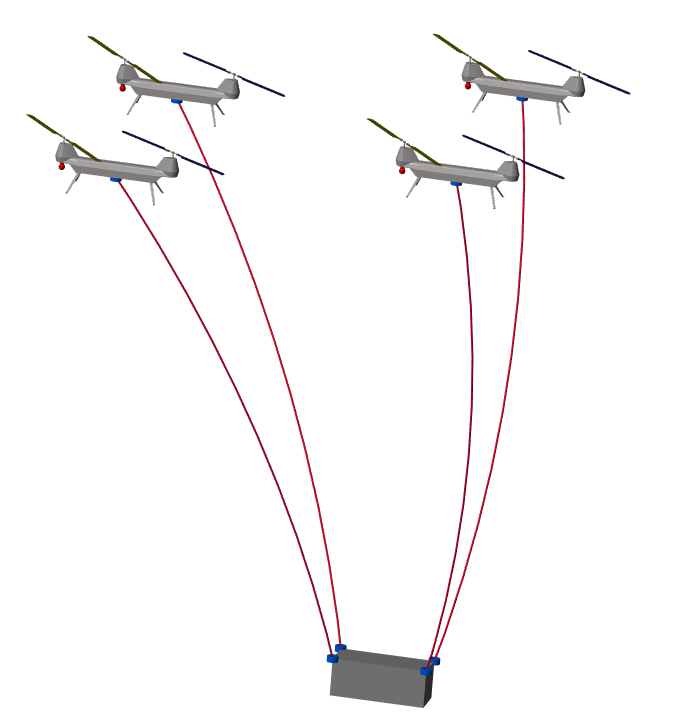
\includegraphics[width = 7cm]{multi_lift.PNG}};
    \draw[-latex] (-2,-2) -- (-3.7,-2) node[above] {飞行方向}; 
    \draw[-latex] (5,-2.5) -- (4,-2.5) node[above] {$X_e$};
    \draw[-latex] (5,-2.5) -- (5.5,-2) node[above] {$Y_e$}; 
    \draw[-latex] (5,-2.5) -- (5,-3.5) node[left] {$Z_e$}; 
    \draw (5,-2.5) node[right, yshift = -0.2cm]{$O_e$};

    \draw[-latex] (0.4,-3.25) -- (-0.5,-3.25) node[below] {$X_{ev,l}$};
    \draw[-latex] (0.4,-3.25) -- (0.9,-2.5) node[left] {$Y_{ev,l}$}; 
    \draw[-latex] (0.4,-3.25) -- (0.4,-4) node[left] {$Z_{ev,l}$}; 
    \draw (0.4,-3.25) node[right, yshift = -0.2cm]{$O_{ev,l}$};

    \draw[-latex] (1.2,1.95) -- (0.5,1.95) node[below] {$X_{ev,1}$};
    \draw[-latex] (1.2,1.95) -- (1.7,2.4) node[left] {$Y_{ev,1}$}; 
    \draw[-latex] (1.2,1.95) -- (1.2,1.2) node[right] {$Z_{ev,1}$}; 
    \draw (1.2,1.95) node[right, yshift = -0.2cm]{$O_{ev,1}$};

\end{tikzpicture}  

% \end{document}
  \caption{本地和机载NED坐标系定义\label{NED}}
\end{figure}

为方便论述,直升机$i$的机载NED坐标系定义为$OXYZ_{ev,i}$,吊挂物的机载NED坐标系定义为$OXYZ_{ev,l}$。图\ref{NED}以四个纵列式直升机协同吊挂为例,给出了吊挂物和直升机1的机载NED坐标系。

\subsubsection{机体坐标系}
机体坐标系又称体轴系,与飞行器固连,用于确定飞行器在空中的姿态,其坐标原点及坐标轴定义如下:
\begin{enumerate}
  \item 坐标原点$O_{b}$位于飞行器质心;
  \item $X$轴$X_{b}$位于飞行器纵向对称面内,指向前;
  \item $Y$轴$Y_{b}$垂直于飞行器纵向对称面,指向右;
  \item $Z$轴$Z_{b}$位于飞行器纵向对称面内,垂直于$X_{b}$轴指向下。
\end{enumerate}

为方便论述,直升机$i$的机体坐标系定义为$OXYZ_{b,i}$,吊挂物机体坐标系定义为$OXYZ_{b,l}$。

\subsubsection{风轴系}
风轴系也叫速度轴系,直升机$i$的风轴系定义为$OXYZ_{V,i}$,吊挂物风轴系定义为$OXYZ_{V,l}$。其坐标原点及坐标轴定义如下:
\begin{enumerate}
  \item 坐标原点$O_V$位于飞行器质心;
  \item $X$轴$X_{V}$沿飞行速度方向;
  \item $Z$轴$Z_{V}$在飞行器纵向对称面内垂直$X_{V}$指向下;
  \item $Y$轴$Y_{V}$由右手定则确定。
\end{enumerate}

\subsubsection{旋翼桨毂轴系}
旋翼桨毂轴系与旋翼桨毂中心固连,其坐标原点及坐标轴定义如下
\begin{enumerate}
  \item 坐标原点$O_h$位于旋翼桨毂中心;
  \item $Z$轴($Z_h$)平行于旋翼轴指向上;
  \item $X$轴($X_h$)位于桨毂平面内且垂直于$Z_h$轴指向后;
  \item 若为右旋旋翼,$Y$轴($Y_h$)由右手定则确定;若为左旋旋翼,$Y$轴($Y_h$)由左手定则确定。
\end{enumerate}
\subsubsection{旋翼旋转轴系}
旋翼旋转轴系记为$OXYZ_r$,其坐标原点及坐标轴定义如下
\begin{enumerate}
  \item 坐标原点$O_r$位于桨毂中心处;
  \item $X$轴($X_r$)为$X_h$轴绕旋翼转向旋转一定方位角后的指向,$X_h$轴初始方位为0 \degree 方位角;
  \item $Z$轴($Z_r$)平行于旋翼轴指向上;
  \item 若为右旋旋翼,$Y$轴($Y_r$)由右手定则确定;若为左旋旋翼,$Y$轴($Y_r$)由左手定则确定。
\end{enumerate}
\subsubsection{桨叶坐标系}
本文中旋翼模型不涉及旋翼的摆振运动,所以相比其他文献,无需定义中心铰坐标系。桨叶坐标系的坐标原点和坐标轴定义如下:
\begin{enumerate}
  \item 坐标原点$O_{bl}$位于挥舞铰上;
  \item $X$轴($X_{bl}$)沿桨叶径向指向外;
  \item $Z$轴($Y_{bl}$)在桨叶挥舞平面内垂直于($X_{bl}$)轴指向上;
  \item 若为右旋旋翼,$Y$轴($Y_{bl}$)由右手定则确定;若为左旋旋翼,$Y$轴($Y_{bl}$)由左手定则确定。
\end{enumerate}
\subsubsection{叶素坐标系}
将桨叶分为$n$个叶素段,则第$i$个叶素的坐标系定义为
\begin{enumerate}
  \item 坐标原点$O_{el,i}$位于第$i$个叶素段中心处;
  \item $X$轴($X_{el,i}$)沿叶素弦线指向前;
  \item $Z$轴($Z_{el,i}$)在叶素对称面内垂直于叶素弦线指向下;
  \item 若为右旋旋翼,$Y$轴($Y_{el,i}$)由右手定则确定;若为左旋旋翼,$Y$轴($Y_{el,i}$)由左手定则确定。
\end{enumerate}
\subsection{坐标系间的转换关系}
为方便下文论述,本节给出了LLA坐标系与ECEF坐标系间的转换关系,ECEF坐标系与NED坐标系间的转换关系、NED坐标系与体轴系间的转换关系、风轴系与体轴系间的转换关系以及欧拉角与四元数间的转换关系。
\subsubsection{LLA坐标系与ECEF坐标系间的转换关系}
\begin{enumerate}
  \item 设LLA坐标系下一点坐标为$(\gamma, \varphi, h)$,则ECEF坐标系下对应坐标为
  \begin{equation}
    \left\{ \begin{gathered}
      {X_{ECEF}} = \left( {N + h} \right)\cos \left( \varphi  \right)\cos \left( \gamma  \right) \hfill \\
      {Y_{ECEF}} = \left( {N + h} \right)\cos \left( \varphi  \right)\sin \left( \gamma  \right) \hfill \\
      {Z_{ECEF}} = \left( {N\left( {1 - {e^2}} \right) + h} \right)\sin \left( \varphi  \right) \hfill \\ 
    \end{gathered}  \right.
  \end{equation}
  \item 反之,ECEF坐标系到LLA坐标系间的转换关系为:
  \begin{equation}
    \left\{ \begin{gathered}
      \gamma  = \arctan \left( {\frac{{{Y_{ECEF}}}}{{{X_{ECEF}}}}} \right) \hfill \\
      \varphi {\text{ = }}\arctan \left( {\frac{Z_{ECEF}}{p}{{\left( {1 - {e^2}\frac{N}{{N + h}}} \right)}^{ - 1}}} \right) \hfill \\
      h = \frac{p}{{\cos \left( \varphi  \right) - N}} \hfill \\ 
    \end{gathered}  \right.
  \end{equation}
  其中,$p = \sqrt{X_{ECEF}^2 + Y_{ECEF}^2}$
\end{enumerate}
\subsubsection{ECEF坐标系与本地NED坐标系间的转换关系}
\begin{enumerate}
  \item 设本地ECEF坐标系原点为$P_{ECEF,0} = (X_{ECEF,0}, Y_{ECEF,0}, Z_{ECEF,0})$,对应的LLA坐标点为$(\gamma_0, \varphi_0, h_0)$。计算点$P_{ECEF}$在ECEF坐标系下的坐标点为$(X_{ECEF}, Y_{ECEF}, Z_{ECEF})$。则$P_{ECEF}$在以$P_{ECEF,0}$为坐标原点的NED坐标系下的坐标为:
  \begin{equation}
    \left[ \begin{gathered}
      n \hfill \\
      e \hfill \\
      d \hfill \\ 
    \end{gathered}  \right] = \underbrace {\left[ {\begin{array}{*{20}{c}}
      { - \sin \left( {{\varphi _0}} \right)\cos \left( {{\gamma _0}} \right)}&{ - \sin \left( {{\varphi _0}} \right)\sin \left( {{\gamma _0}} \right)}&{\cos \left( {{\varphi _0}} \right)} \\ 
      { - \sin \left( {{\gamma _0}} \right)}&{\cos \left( {{\gamma _0}} \right)}&0 \\ 
      {-\cos \left( {{\varphi _0}} \right)\cos \left( {{\gamma _0}} \right)}&{-\cos \left( {{\varphi _0}} \right)\sin \left( {{\gamma _0}} \right)}&{-\sin \left( {{\varphi _0}} \right)} 
    \end{array}} \right]}_S\left[ \begin{gathered}
      \Delta x \hfill \\
      \Delta y \hfill \\
      \Delta z \hfill \\ 
    \end{gathered}  \right]
  \end{equation}
  其中,$\Delta x = X_{ECEF} - X_{ECEF,0}$,$\Delta y = Y_{ECEF} - Y_{ECEF,0}$,$\Delta z = Z_{ECEF} - Z_{ECEF,0}$。
  \item 反之,
  \begin{equation}
    \left[ \begin{gathered}
      \Delta x \hfill \\
      \Delta y \hfill \\
      \Delta z \hfill \\ 
    \end{gathered}  \right] = {S^{ - 1}}\left[ \begin{gathered}
      n \hfill \\
      e \hfill \\
      d \hfill \\ 
    \end{gathered}  \right]
  \end{equation}
\end{enumerate}

\subsubsection{机载NED坐标系与体轴系间的转换关系}
机载NED坐标系依次绕Z-Y-X轴做欧拉旋转,得到体轴系。以直升机$i$为例,坐标系$OXYZ_{ev,i}$与坐标系$OXYZ_{b,i}$之间的转换关系为
\begin{equation}
  \left[ \begin{gathered}
    {X_{b,i}} \hfill \\
    {Y_{b,i}} \hfill \\
    {Z_{b,i}} \hfill \\ 
  \end{gathered}  \right] = \underbrace {\underbrace {\left[ {\begin{array}{*{20}{c}}
    1&0&0 \\ 
    0&{\cos {\phi _i}}&{\sin {\phi _i}} \\ 
    0&{ - \sin {\phi _i}}&{\cos {\phi _i}} 
  \end{array}} \right]}_{{{\mathbf{R}}_x}}\underbrace {\left[ {\begin{array}{*{20}{c}}
    {\cos {\theta _i}}&0&{ - \sin {\theta _i}} \\ 
    0&1&0 \\ 
    {\sin {\theta _i}}&0&{\cos {\theta _i}} 
  \end{array}} \right]}_{{{\mathbf{R}}_y}}\underbrace {\left[ {\begin{array}{*{20}{c}}
    {\cos {\psi _i}}&{\sin {\psi _i}}&0 \\ 
    { - \sin {\psi _i}}&{\cos {\psi _i}}&0 \\ 
    0&0&1 
  \end{array}} \right]}_{{{\mathbf{R}}_z}}}_{{{\mathbf{R}}_{bi/evi}}}\left[ \begin{gathered}
    {X_{ev,i}} \hfill \\
    {Y_{ev,i}} \hfill \\
    {Z_{ev,i}} \hfill \\ 
  \end{gathered}  \right]
\end{equation}
其中,$\mathbf{R}_{bi/evi}$称为直升机$i$机载NED坐标系到体轴系的转换矩阵。

此外,
\begin{enumerate}
  \item 偏航角$\psi_i$为机载坐标系绕$Z$轴旋转过的角度,即机载NED坐标系$X_{ev,i}$轴与体轴系$X_{b,i}$轴在机载NED坐标系$X_{ev,i}Y_{ev,i}$平面的投影,经过$\mathbf{R}_z$转换后得到中间坐标系;
  \item 俯仰角$\theta_i$为中间坐标系绕$Y$轴旋转过的角度,经过$\mathbf{R}_y$转换后得到二次中间坐标系;
  \item 滚转角$\phi_i$为二次中间坐标系绕$X$轴旋转的角度,旋转矩阵记作$\mathbf{R}_x$。
\end{enumerate}

图\ref{body}以直升机1为例,给出了机载NED坐标系与体轴系的转换关系及姿态角定义。

\begin{figure}[htb!]
  \subfloat[绕$Z$轴旋转]{% \documentclass{article}
% \usepackage{xeCJK}
% \usepackage{tikz}
% \usetikzlibrary{decorations.pathreplacing, calligraphy}
% \usetikzlibrary{quotes,angles}
% \begin{document}
\begin{tikzpicture}
    \node at (0,0) {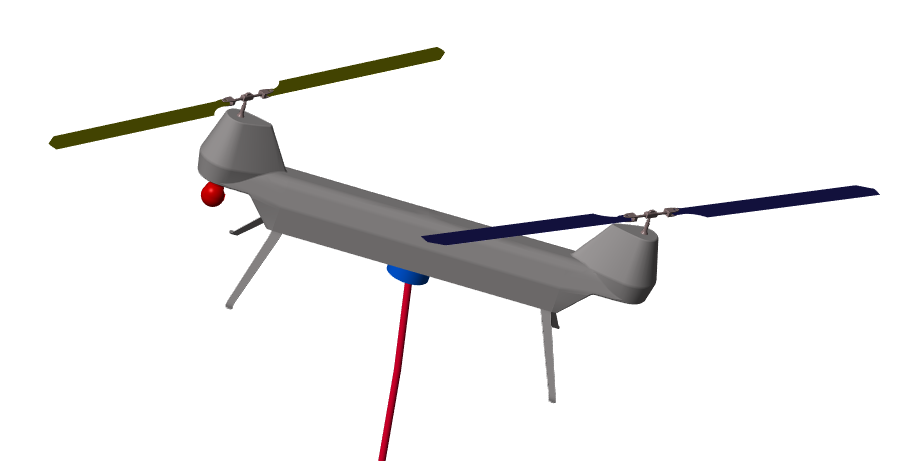
\includegraphics[width = 5cm]{tandem.PNG}};
    \draw[-latex] (-1,-2) -- (-2.5,-2) node[above] {飞行方向}; 
    %机载NED坐标系 
    \draw[-latex] (-0.3,-0.1) -- (-3.,-0.1) node[below] {$X_{ev,1}$};
    \draw[-latex] (-0.3,-0.1) -- (1.0,1.5) node[left] {$Y_{ev,1}$}; 
    \draw[-latex] (-0.3,-0.1) -- (-0.3,-2) node[right,yshift = 0.5cm] {$Z_{ev,1}$}; 
    \draw (-0.3,-0.1) node[right, yshift = -0.2cm]{$O_{ev,1}$} node[right, yshift = -0.6cm]{$O_{b,1}^z$};
    % 绕z轴旋转后的坐标系
    \draw[-latex] (-0.3,-0.1) -- (-3.,0.35) node[above] {$X_{b,1}^z$};
    \draw[-latex] (-0.3,-0.1) -- (1.5,1.4) node[right] {$Y_{b,1}^z$}; 
    \draw[-latex] (-0.3,-0.1) -- (-0.3,-2) node[right] {$Z_{b,1}^z$}; 
    \draw
    (-3.,0.35) coordinate (a)
    (-0.3, -0.1) coordinate (b)
    (-3.,-0.1) coordinate (c)
    pic["$\psi_1$", draw=orange, <-, angle eccentricity=1.2, angle radius=1.8cm]
    {angle=a--b--c};
\end{tikzpicture}  

% \end{document}}\quad
  \subfloat[绕$Y$轴旋转]{% \documentclass{article}
% \usepackage{xeCJK}
% \usepackage{tikz}
% \usetikzlibrary{decorations.pathreplacing, calligraphy}
% \usetikzlibrary{quotes,angles}
% \begin{document}
\begin{tikzpicture}
    \node at (0,0) {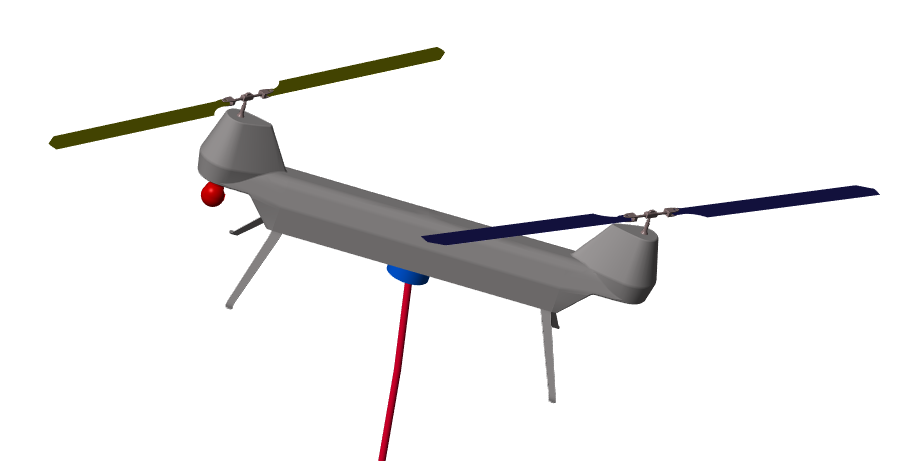
\includegraphics[width = 5cm]{tandem.PNG}};
    \draw[-latex] (-1,-2) -- (-2.5,-2) node[above] {飞行方向}; 
    \draw (-0.3,-0.1) node[right, yshift = -0.2cm]{$O_{b,1}^z$} node[right, yshift = -0.6cm]{$O_{b,1}^{y}$};
    % 绕z轴旋转
    \draw[-latex] (-0.3,-0.1) -- (-3.,0.35) node[below] {$X_{b,1}^z$};
    \draw[-latex] (-0.3,-0.1) -- (1.5,1.4) node[right] {$Y_{b,1}^z$}; 
    \draw[-latex] (-0.3,-0.1) -- (-0.3,-2) node[right] {$Z_{b,1}^z$}; 
    % 绕y轴旋转
    \draw[-latex] (-0.3,-0.1) -- (-3.,0.7) node[above] {$X_{b,1}^y$};
    \draw[-latex] (-0.3,-0.1) -- (1.5,1.4) node[right, yshift = -0.5cm] {$Y_{b,1}^y$}; 
    \draw[-latex] (-0.3,-0.1) -- (-0.65,-2) node[left,yshift = 0.4cm] {$Z_{b,1}^y$}; 
    \draw
    (-3.,0.7) coordinate (a)
    (-0.3, -0.1) coordinate (b)
    (-3.,0.35) coordinate (c)
    pic["$\theta_1$", draw=orange, <-, angle eccentricity=1.2, angle radius=1.8cm]
    {angle=a--b--c};
\end{tikzpicture}  

% \end{document}}
  \subfloat[绕$X$轴旋转]{% \documentclass{article}
% \usepackage{xeCJK}
% \usepackage{tikz}
% \usetikzlibrary{decorations.pathreplacing, calligraphy}
% \usetikzlibrary{quotes,angles}
% \begin{document}
\begin{tikzpicture}
    \node at (0,0) {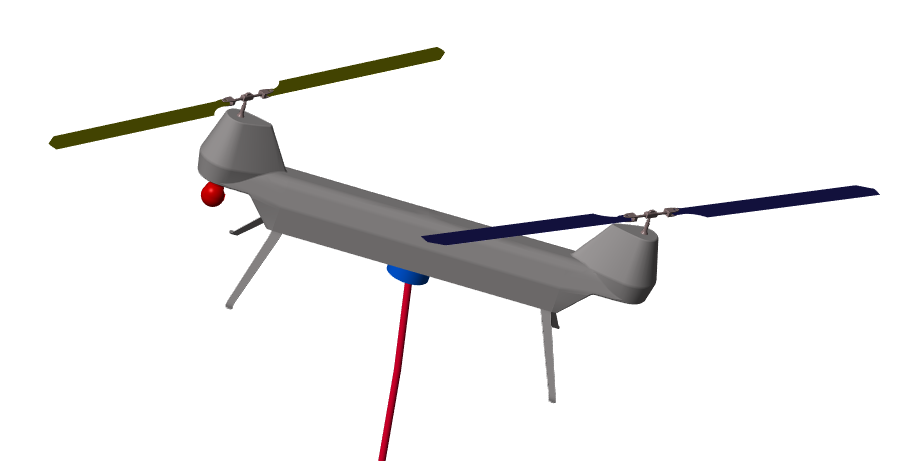
\includegraphics[width = 5cm]{tandem.PNG}};
    \draw[-latex] (-1,-2) -- (-2.5,-2) node[above] {飞行方向}; 
    \draw (-0.3,-0.1) node[right, yshift = -0.2cm]{$O_{b,1}^y$} node[right, yshift = -0.6cm]{$O_{b,1}$};
    % 绕y轴旋转
    \draw[-latex] (-0.3,-0.1) -- (-3.,0.7) node[above] {$X_{b,1}^y$};
    \draw[-latex] (-0.3,-0.1) -- (1.5,1.4) node[right] {$Y_{b,1}^y$}; 
    \draw[-latex] (-0.3,-0.1) -- (-0.65,-2) node[right,yshift = 0.4cm] {$Z_{b,1}^y$}; 
     % 绕x轴旋转
     \draw[-latex] (-0.3,-0.1) -- (-3.,0.7) node[below] {$X_{b,1}$};
     \draw[-latex] (-0.3,-0.1) -- (1.5,1.0) node[right] {$Y_{b,1}$}; 
     \draw[-latex] (-0.3,-0.1) -- (-0.95,-1.9) node[left,yshift = 0.4cm] {$Z_{b,1}$};   
     \draw
    (1.5,1.0) coordinate (a)
    (-0.3, -0.1) coordinate (b)
    (1.5,1.4) coordinate (c)
    pic["$\phi_1$", draw=orange, <-, angle eccentricity=1.2, angle radius=1.5cm]
    {angle=a--b--c};
\end{tikzpicture}  

% \end{document}}
  \caption{机载NED坐标系转到体轴系及姿态角定义\label{body}}
\end{figure}

\subsubsection{风轴系与体轴系间的转换关系}
定义侧滑角$\beta$为速度矢量与$X_bO_bY_b$平面夹角,右侧滑为正。迎角$\alpha$为速度矢量在$X_bO_bZ_b$平面的投影与$O_bX_b$轴的夹角,速度矢量在$X_bO_bY_b$平面下方时迎角为正。

风轴系与体轴系间的转换关系为
\begin{equation}
  \left[ \begin{gathered}
    {X_b} \hfill \\
    {Y_b} \hfill \\
    {Z_b} \hfill \\ 
  \end{gathered}  \right] = \underbrace {\underbrace {\left[ {\begin{array}{*{20}{c}}
    {\cos \alpha }&0&{ - \sin \alpha } \\ 
    0&1&0 \\ 
    {\sin \alpha }&0&{\cos \alpha } 
  \end{array}} \right]}_{{{\mathbf{R}}_\alpha }}\underbrace {\left[ {\begin{array}{*{20}{c}}
    {\cos \beta }&{ - \sin \beta }&0 \\ 
    {\sin \beta }&{\cos \beta }&0 \\ 
    0&0&1 
  \end{array}} \right]}_{{{\mathbf{R}}_\beta }}}_{{{\mathbf{R}}_{b/V}}}\left[ \begin{gathered}
    {X_V} \hfill \\
    {Y_V} \hfill \\
    {Z_V} \hfill \\ 
  \end{gathered}  \right]
\end{equation}

\begin{figure}[htb!]
  \subfloat[桨轴前倾角]{% \documentclass{article}
% \usepackage{xeCJK}
% \usepackage{tikz}
% \usetikzlibrary{decorations.pathreplacing, calligraphy}
% \usetikzlibrary{quotes,angles}
% \begin{document}
\begin{tikzpicture}
    % 体轴系
    \draw[-latex] (-0.3,-0.1) -- (-3.,-0.1) node
    [above] {$X_{b,1}$};
    \draw[-latex] (-0.3,-0.1) -- (1.5,1.4) node[right] {$Y_{b,1}$}; 
    \draw[-latex] (-0.3,-0.1) -- (-0.3,-2) node[right] {$Z_{b,1}$}; 
    %桨毂轴系
    \draw[-latex] (-0.3,-0.1) -- (2.5,0.5) node[above] {$X_{h}$};
    \draw[-latex] (-0.3,-0.1) -- (1.5,1.4) node[right,yshift = 0.4cm] {$Y_{h}$}; 
    \draw[-latex] (-0.3,-0.1) -- (-0.8,2) node[left] {$Z_{h}$};
    % 辅助线
    \draw[dash dot](-0.3,-0.1) -- (2.5,-0.1);
    \draw[dash dot](-0.3,-0.1) -- (-0.3,2);
    \draw
    (-0.3,2) coordinate (a)
    (-0.3, -0.1) coordinate (b)
    (-0.8,2) coordinate (c)
    pic["$\delta$", draw=orange, ->, angle eccentricity=1.2, angle radius=1.5cm]
    {angle=a--b--c};
\end{tikzpicture}  

% \end{document}}\quad
  \subfloat[旋翼旋转轴系]{% \documentclass{article}
% \usepackage{xeCJK}
% \usepackage{tikz}
% \usetikzlibrary{decorations.pathreplacing, calligraphy}
% \usetikzlibrary{quotes,angles}
% \begin{document}
\begin{tikzpicture}
    \node at (1.1,-1.3) {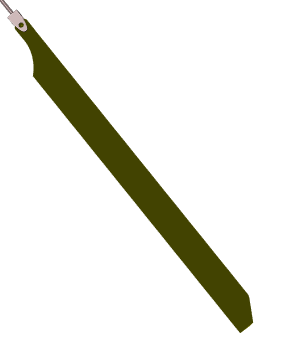
\includegraphics[width = 2.2cm]{blade.png}};
    \draw[dash dot](-2,0)--(1,0);
    \draw[dash dot](0,-2)--(0,1);
    \draw[-latex] -> (0,0)--(0,-3.0) node[left]{$X_h$};
    \draw[-latex] -> (0,0)--(1.8,0) node[above]{$Y_h$};
    \draw[-latex] -> (0,0)--(2.14,-2.7) node[left]{$X_r$};
    \draw[-latex] -> (0,0)--(1.5,1.1) node[above]{$Y_r$};
    \draw 
    (0,-4)coordinate(a)
    (0,0)coordinate(b)
    (2.14,-2.7)coordinate(c)
    pic["$\psi_r$", draw=orange, ->, angle eccentricity=1.2, angle radius=1.5cm]
    {angle=a--b--c};

\end{tikzpicture}  

% \end{document}}\quad
  \subfloat[桨叶坐标系]{% \documentclass{article}
% \usepackage{xeCJK}
% \usepackage{tikz}
% \usetikzlibrary{decorations.pathreplacing, calligraphy}
% \usetikzlibrary{quotes,angles}
% \begin{document}
\begin{tikzpicture}
    \node at (0,0) {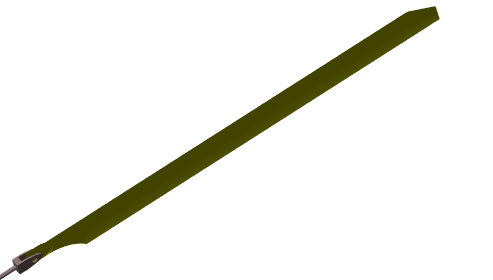
\includegraphics[width = 3cm]{blade1.png}};
    \draw[-latex](-1.5,-0.85)--(2,-0.85) node[below]{$X_r$};
    \draw[-latex](-1.5,-0.85)--(-1.5,1) node[above]{$Z_r$};
    \draw[-latex](-1.5,-0.85)--(1.8,1.25) node[above]{$X_{bl}$};
    \draw[-latex](-1.5,-0.85)--(-2.6,1) node[left]{$Z_{bl}$};
    \draw 
    (2,-0.85)coordinate(a)
    (-1.5,-0.85)coordinate(b)
    (1.8,1.25)coordinate(c)
    pic["$\beta_{bl}$", draw=orange, ->, angle eccentricity=1.2, angle radius=1.5cm]
    {angle=a--b--c};

\end{tikzpicture}  

% \end{document}}\quad\quad
  \subfloat[叶素坐标系]{% \documentclass{article}
% \usepackage{xeCJK}
% \usepackage{tikz}
% \usetikzlibrary{decorations.pathreplacing, calligraphy}
% \usetikzlibrary{quotes,angles}
% \begin{document}
\begin{tikzpicture}
    \node at (0,0) {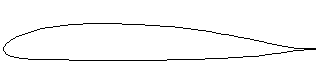
\includegraphics[width = 4cm, angle = -30]{OA212.png}};
    \draw[-latex](-0.5,0.2)--(-2.5,0.2) node[below]{$Y_{bl}$};
    \draw[-latex](-0.5,0.2)--(-0.5,2) node[left]{$Z_{bl}$};
    \draw[-latex](-0.5,0.2)--(-2.5,1.2) node[above]{$X_{el,i}$};
    \draw[-latex](-0.5,0.2)--(-1.1,-1.2) node[left]{$Z_{el,i}$};
    \draw 
    (-2.5,1.2)coordinate(a)
    (-0.5,0.2)coordinate(b)
    (-2.5,0.2)coordinate(c)
    pic["$\theta_{el,i}$", draw=orange, <-, angle eccentricity=1.2, angle radius=1.5cm]
    {angle=a--b--c};

\end{tikzpicture}  

% \end{document}}
  \caption{体轴系、桨毂轴系、旋翼旋转轴系、桨叶坐标系、叶素坐标系间的转换关系\label{rotor}}
\end{figure}
\subsubsection{体轴系与桨毂轴系间的转换关系}
定义桨轴前倾角为$\delta$,见图\ref{rotor}(a)。以右旋旋翼为例,体轴系与桨毂轴系间的欧拉角为$(0, \pi-\delta, 0)$,对应的转换关系为
\begin{equation}
  \left[ \begin{gathered}
    {X_h} \hfill \\
    {Y_h} \hfill \\
    {Z_h} \hfill \\ 
  \end{gathered}  \right] = \underbrace {\left[ {\begin{array}{*{20}{c}}
    {\cos \delta }&0&{\sin \delta } \\ 
    0&1&0 \\ 
    { - \sin \delta }&0&{\cos \delta } 
  \end{array}} \right]\left[ {\begin{array}{*{20}{c}}
    { - 1}&0&0 \\ 
    0&1&0 \\ 
    0&0&{ - 1} 
  \end{array}} \right]}_{{{\mathbf{R}}_{h/b}}}\left[ \begin{gathered}
    {X_b} \hfill \\
    {Y_b} \hfill \\
    {Z_b} \hfill \\ 
  \end{gathered}  \right]
\end{equation}
\subsubsection{桨毂轴系与旋翼旋转轴系间的转换关系}
在方位角为$\psi_r$时,见图\ref{rotor}(b),旋翼桨毂轴系与旋转轴系之间的欧拉角为$(0, 0, \psi_r)$,对应的转换关系为
\begin{equation}
  \left[ \begin{gathered}
    {X_{r}} \hfill \\
    {Y_{r}} \hfill \\
    {Z_{r}} \hfill \\ 
  \end{gathered}  \right] = \underbrace {\left[ {\begin{array}{*{20}{c}}
    \cos \psi_r&\sin \psi_r&0 \\ 
    -\sin \psi_r&\cos \psi_r&0 \\ 
    0&0&1
  \end{array}} \right]}_{{{\mathbf{R}}_{r/h}}}\left[ \begin{gathered}
    {X_h} \hfill \\
    {Y_h} \hfill \\
    {Z_h} \hfill \\ 
  \end{gathered}  \right]
\end{equation}

\subsubsection{旋翼旋转轴系与桨叶坐标系间的转换关系}
当挥舞角为$\beta_{bl}$时,见图\ref{rotor}(c),旋翼旋转轴系与桨叶坐标系间的欧拉角为$(0, -\beta_{bl}, 0)$,对应的转换关系为
\begin{equation}
  \left[ \begin{gathered}
    {X_{bl}} \hfill \\
    {Y_{bl}} \hfill \\
    {Z_{bl}} \hfill \\ 
  \end{gathered}  \right] = \underbrace {\left[ {\begin{array}{*{20}{c}}
    {\cos {\beta _{bl}}}&0&{\sin {\beta _{bl}}} \\ 
    0&1&0 \\ 
    { - \sin {\beta _{bl}}}&0&{\cos {\beta _{bl}}} 
  \end{array}} \right]}_{{{\mathbf{R}}_{bl/r}}}\left[ \begin{gathered}
    {X_r} \hfill \\
    {Y_r} \hfill \\
    {Z_r} \hfill \\ 
  \end{gathered}  \right]
\end{equation}
\subsubsection{桨叶坐标系与叶素坐标系间的转换关系}
桨叶坐标系绕$Z$轴旋转90 \degree ,绕$X$轴旋转180 \degree 得到中间坐标系。当第$i$个叶素桨距为$\theta_{el,i}$时,见图\ref{rotor}(d),中间坐标系与叶素坐标系间的欧拉角为$(\theta_{el,i}, 0, 0)$,对应的转换关系为
\begin{equation}
  \left[ \begin{gathered}
    {X_{el,i}} \hfill \\
    {Y_{el,i}} \hfill \\
    {Z_{el,i}} \hfill \\ 
  \end{gathered}  \right] = \underbrace {\left[ {\begin{array}{*{20}{c}}
    1&0&0 \\ 
    0&{\cos {\theta _{el,i}}}&{\sin {\theta _{el,i}}} \\ 
    0&{ - \sin {\theta _{el,i}}}&{\cos {\theta _{el,i}}} 
  \end{array}} \right]\left[ {\begin{array}{*{20}{c}}
    1&0&0 \\ 
    0&{ - 1}&0 \\ 
    0&0&{ - 1} 
  \end{array}} \right]\left[ {\begin{array}{*{20}{c}}
    0&1&0 \\ 
    { - 1}&0&0 \\ 
    0&0&1 
  \end{array}} \right]}_{{{\mathbf{R}}_{el,i/bl}}}\left[ \begin{gathered}
    {X_{bl}} \hfill \\
    {Y_{bl}} \hfill \\
    {Z_{bl}} \hfill \\ 
  \end{gathered}  \right]
\end{equation}

\subsubsection{欧拉角与四元数间的转换关系}
四元数在一些方面优于欧拉角和旋转矩阵。任意一个三维空间中的定向都可以被表示为一个绕某个特定轴的旋转。给定旋转轴及旋转角度,很容易把其他形式的旋转表示成四元数或者把四元数转换成其他形式。四元数可以用于稳定的、经常性的旋转插值,这些在欧拉角中很难实现。

一个四元数可以被定义为如下形式:
\section{直升机模型}
纵列式直升机建模方法参考\cite{mahmuddin2017rotor,Duan2021Accepted}。每个直升机有30个状态量,包括12个刚体运动状态量、9个前旋翼状态量和9个后旋翼状态量。如下:
\begin{equation}
  \left\{ \begin{array}{l}
      {{\bf{x}}_{rigid,i}} = \left[ {{u_i},{v_i},{w_i},{p_i},{q_i},{r_i},{\phi _i},{\theta _i},{\psi _i},{\;^e}{{\bf{P}}_i}^T} \right]\\
      {{\bf{x}}_{front,i}} = \left[ {{\beta _{0,F}},{\beta _{1s,F}},{\beta _{1c,F}},{{\dot \beta }_{0,F}},{{\dot \beta }_{1s,F}},{{\dot \beta }_{1c,F}},{\lambda _{0,F}},{\lambda _{1s,F}},{\lambda _{1c,F}}} \right]\\
      {{\bf{x}}_{rear,i}} = \left[ {{\beta _{0,R}},{\beta _{1s,R}},{\beta _{1c,R}},{{\dot \beta }_{0,R}},{{\dot \beta }_{1s,R}},{{\dot \beta }_{1c,R}},{\lambda _{0,R}},{\lambda _{1s,R}},{\lambda _{1c,R}}} \right]\\
      {{\bf{x}}_i} = \left[ {{{\bf{x}}_{rigid,i}}\;{{\bf{x}}_{front,i}}\;{{\bf{x}}_{rear,i}}} \right]^T
      \end{array} \right.
\end{equation}
其中, $\left[ {u_i,v_i,w_i} \right]$和$\left[ {p_i,q_i,r_i} \right]$分别为直升机$i$在其体轴系下的线速度和角速度,$\left[ {{\phi _i},{\theta _i},{\psi _i}} \right]$是轴系${x_e}{y_e}{z_e}$和${x_{ib}}{y_{ib}}{z_{ib}}$间的欧拉角,$\left[ {{\beta _0},{\beta _{1s}},{\beta _{1c}}} \right]$和$\left[ {{{\dot \beta }_0},{{\dot \beta }_{1s}},{{\dot \beta }_{1c}}} \right]$分别为桨叶挥舞角和挥舞角速度写成傅里叶级数时的系数,$\left[ {{\lambda _0},{\lambda _{1s}},{\lambda _{1c}}} \right]$是旋翼入流速度写成傅里叶级数形式时的系数。
\subsection{旋翼气动模型}
\subsubsection{旋翼挥舞模型}
\subsubsection{旋翼入流模型}
\subsubsection{桨叶气动力模型}
\subsection{机身气动模型}
\subsection{直升机动力学模型}

\section{柔性吊索模型}
吊索的作用是连接直升机和吊挂物。如图\ref{fig:chap_2_4_2_1}所示,假定吊索质量集中于$n$个质点,质点之间通过弹簧阻尼系统相连。吊索与直升机相连于吊点A,与吊挂物相连于吊点B。单个质点受到重力、气动阻力、张力的共同作用。设吊索总质量为$m_c$,初始长度为$l^{c0}$,刚度系数为$K_c$,阻尼系数为$C_c$。则各个质点的质量为
\begin{equation}
  m_k^{\text{c}} = \frac{{{m_{\text{c}}}}}{n}\;\;\;\;\;k = 1,2, \cdots ,n
\end{equation}

每段吊索的初始长度为
\begin{equation}
  l_k^{{\rm{c0}}} = \left\{ \begin{array}{l}
    \frac{{{l_{{\rm{c}}0}}}}{n}\;\;\;\;\;\;\;\;\;\;k = 1,2, \cdots ,n - 1\\
    \frac{{{l_{{\rm{c}}0}}}}{{2n}}\;\;\;\;\;\;\;\;\;\;k = 0,n
    \end{array} \right.
\end{equation}

设地轴系下吊点A和B的位置分别为$\mathbf{x}_\text{A}$和$\mathbf{x}_\text{B}$,第$k$个质点的空间位置为$\mathbf{x}_k^{\text{c}}$, 则每段吊索在地轴系下的投影向量为
\begin{equation}
  \mathbf{R}_k^\text{c} = \left\{ \begin{array}{l}
    \mathbf{x}_{k-1}^{\text{c}} - \mathbf{x}_k^{\text{c}}\;\;\;\;\;\;\;\;\;\;k = 1,2, \cdots ,n - 1\\
    \mathbf{x}_{1}^{\text{c}} - \mathbf{x}_{\text{A}}\;\;\;\;\;\;\;\;\;\;\;\;k = 0\\
    \mathbf{x}_{\text{B}} - \mathbf{x}_{n}^{\text{c}}\;\;\;\;\;\;\;\;\;\;\;\;k = n
    \end{array} \right.
\end{equation}

每段吊索的实际长度为
\begin{equation}
  l_k^{\text{c}} = \left| {{\mathbf{R}}_k^{\text{c}}} \right|
\end{equation}

每根吊索的伸长率为
\begin{equation}
  \dot l_k^{\text{c}} = \frac{1}{{l_k^{\text{c}}}}{\left( {\dot {\mathbf{R}}_k^{\text{c}}} \right)^T}{\mathbf{R}}_k^{\text{c}},\;\;\;\;\;\;\;k = 0,1, \cdots n
\end{equation}

每段吊索的张力为
\begin{equation}
  F_k^{\text{c}} = \left\{ \begin{gathered}
    {K_{\text{c}}}\left( {l_k^{\text{c}} - l_k^{{\text{c}}0}} \right) + {C_{\text{c}}}\;\dot l_k^{\text{c}}\;\;\;\;\;\;\;\;l_k^{\text{c}} > l_k^{{\text{c}}0},\;\dot l_k^{\text{c}} > 0,\;\;k = 0,1, \cdots n \hfill \\
    {K_{\text{c}}}\left( {l_k^{\text{c}} - l_k^{{\text{c}}0}} \right)\;\;\;\;\;\;\;\;\;\;\;\;\;\;\;\;\;\;l_k^{\text{c}} > l_k^{{\text{c}}0},\;\dot l_k^{\text{c}} \leqslant 0,\;\;k = 0,1, \cdots n \hfill \\
    0\;\;\;\;\;\;\;\;\;\;\;\;\;\;\;\;\;\;\;\;\;\;\;\;\;\;\;\;\;\;\;\;\;l_k^{\text{c}} \leqslant l_k^{{\text{c}}0},\;\;k = 0,1, \cdots n \hfill \\ 
  \end{gathered}  \right.
\end{equation}

与重量类似,假定吊索气动阻力集中于$n$个质点,设吊索单位长度气动阻力系数为$C_{\text{Dc}}$,则第$k$段吊索气动阻力$D_{k}^\text{a}$为
\begin{equation}
  D_k^{\text{a}} = \left\{ \begin{gathered}
    \frac{1}{2}\rho {C_{{\text{D}}c}}\frac{{l_{k - 1}^{\text{c}} + l_k^{\text{c}}}}{2}{\left| {\dot{\mathbf{x}}_k^{\text{c}} - {\mathbf{V}}_k^{gc}} \right|^2},\;\;\;\;\;\;\;\;\;k = 2,3, \cdots ,n - 1 \hfill \\
    \frac{1}{2}\rho {C_{{\text{D}}c}}\left( {l_0^{\text{c}} + \frac{{l_1^{\text{c}}}}{2}} \right){\left| {\dot{\mathbf{x}}_1^{\text{c}} - {\mathbf{V}}_1^{gc}} \right|^2},\;\;\;\;\;\;\;\;k = 1 \hfill \\
    \frac{1}{2}\rho {C_{{\text{D}}c}}\left( {l_n^{\text{c}} + \frac{{l_{n - 1}^{\text{c}}}}{2}} \right){\left| {\dot {\mathbf{x}}_n^{\text{c}} - {\mathbf{V}}_n^{gc}} \right|^2},\;\;\;\;\;\;k = n \hfill \\ 
  \end{gathered}  \right.
\end{equation}
其中,$\mathbf{V}_k^{gc}$为第$k$个质点处当地的气流对地速度。

基于此,可得第$k$个质点的动力学方程为
\begin{equation}
  {\mathbf{\ddot x}}_k^{\text{c}} = \frac{{F_k^{\text{c}}}}{{m_k^{\text{c}}l_k^{\text{c}}}}{\mathbf{R}}_k^{\text{c}} - \frac{{F_{k - 1}^{\text{c}}}}{{m_{k - 1}^{\text{c}}l_{k - 1}^{\text{c}}}}{\mathbf{R}}_{k - 1}^{\text{c}} - \frac{{D_k^{\text{a}}}}{{m_k^{\text{c}}\left| {\dot {\mathbf{x}}_k^{\text{c}} - {\mathbf{V}}_k^{{\text{gc}}}} \right|}}\left( {\dot {\mathbf{x}}_k^{\text{c}} - {\mathbf{V}}_k^{{\text{gc}}}} \right) + \left[ \begin{gathered}
    0 \hfill \\
    0 \hfill \\
    g \hfill \\ 
  \end{gathered}  \right],\;\;\;\;\;k = 1,2, \cdots n
\end{equation}
其中,$g$为重力加速度。

则地轴系下吊索对直升机和吊挂物的作用力$\mathbf{F}_{\text{Ac}}$和$\mathbf{F}_{\text{Bc}}$分别为
\begin{equation}
  \left\{ \begin{gathered}
    {{\mathbf{F}}_{{\text{Ac}}}} = \frac{{F_0^{\text{c}}}}{{l_0^{\text{c}}}}{\mathbf{R}}_0^c \hfill \\
    {{\mathbf{F}}_{{\text{Bc}}}} = {\text{ - }}\frac{{F_n^{\text{c}}}}{{l_n^{\text{c}}}}{\mathbf{R}}_n^c \hfill \\ 
  \end{gathered}  \right.
\end{equation}

\begin{figure}
  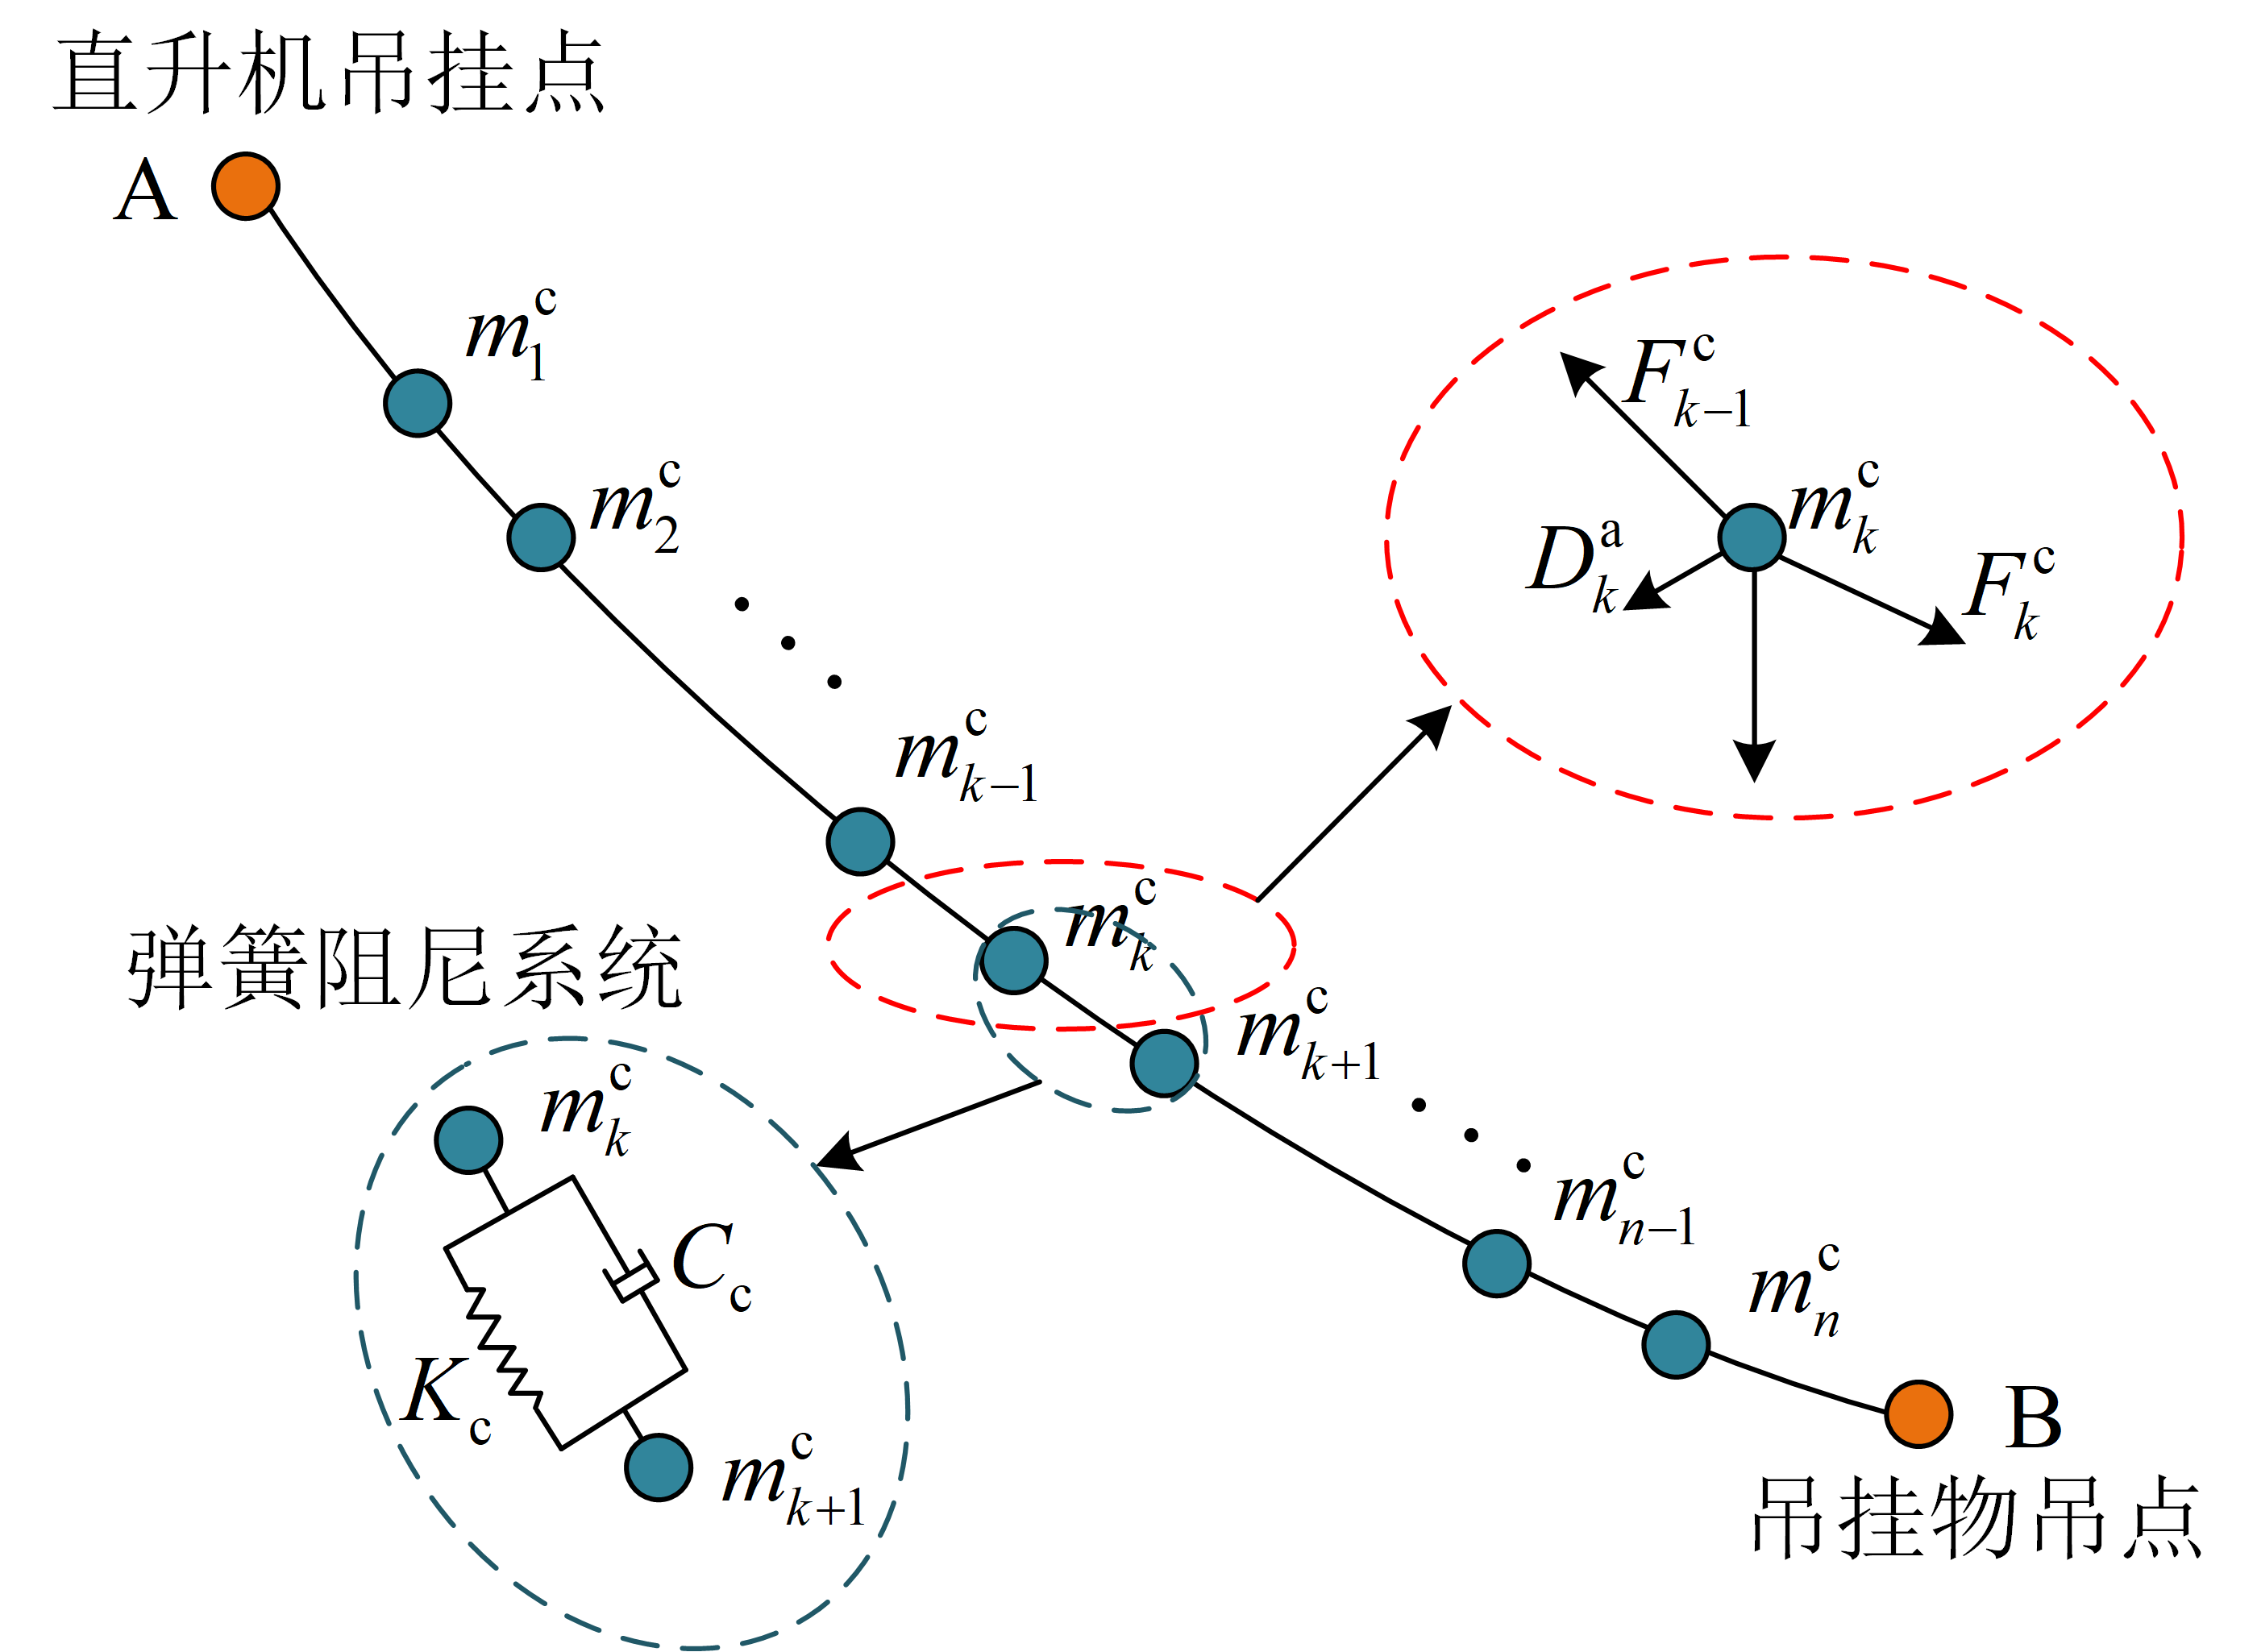
\includegraphics[width=8cm]{fig/figure_chap2/chap_2_4_2_1.png}
  \caption{吊索拉力、吊索角度定义}
  \label{fig:chap_2_4_2_1}
\end{figure}

\section{吊挂物模型}
假设吊挂物体轴系$x_Ly_Lz_L$原点位于吊挂物重心处,则基于牛顿-欧拉方法,吊挂物的动力学方程可以写为
\begin{equation}
  {{\bf{M}}_{\bf{L}}}{\dot{\bf{x}}} + {{\bf{C}}_{\bf{L}}}{\bf{x}} = {{\bf{g}}_L} + {{\bf{M}}_c} + {{\bf{M}}_{aero}}
  \label{equation:chap_4_1}
\end{equation}
其中,$\mathbf{M}_{aero}$是气动力、力矩,$\mathbf{M}_{c}$是由吊索引起的力和力矩,此外
\begin{equation}
  \left\{ {\begin{array}{*{20}{c}}
      {{{\bf{M}}_L} = \left[ {\begin{array}{*{20}{c}}
      {{{\bf{I}}_{3 \times 3}}}&{}&{}&{}\\
      {}&{{{\bf{I}}_{3 \times 3}}}&{}&{}\\
      {}&{}&{{m_L}{{\bf{I}}_{3 \times 3}}}&{}\\
      {}&{}&{}&{{{\bf{J}}_L}}
      \end{array}} \right]}\\
      {{{\bf{C}}_L}{\bf{x}} = \left[ {\begin{array}{*{20}{c}}
      {^e{{\bf{R}}_L}{\bf{V}}}\\
      {^{Euler}{{\bf{R}}_{Body}}{\bm{\omega }}}\\
      {{{\bf{0}}_{3 \times 3}}}\\
      {{\bm{\omega }} \times {{\bf{J}}_L}{\bm{\omega }}}
      \end{array}} \right]}\\
      {{g_L} = \left[ {\begin{array}{*{20}{c}}
      \begin{array}{l}
      \;\;\;\;\;\;\;\;\;{{\bf{0}}_{3 \times 1}}\\
      \;\;\;\;\;\;\;\;\;{{\bf{0}}_{3 \times 1}}\\
      ^L{{\bf{R}}_e}{\left[ {\begin{array}{*{20}{c}}
      0&0&{{m_L}g}
      \end{array}} \right]^T}
      \end{array}\\
      {{{\bf{0}}_{3 \times 1}}}
      \end{array}} \right]}\\
      {\dot{\bf{x}} = {{\left[ {\begin{array}{*{20}{c}}
      {^e{{\dot{\bf{P}}}_L}^T}&{\left[ {{{\dot \phi }_L},{{\dot \theta }_L},{{\dot \psi }_L}} \right]}&{\dot{\bf{V}}^T}&{{\bm{\dot \omega ^T}}}
      \end{array}} \right]}^T}\;}\\
      {{\bf{x}} = {{\left[ {\begin{array}{*{20}{c}}
      {^e{{\bf{P}}_L^T}}&{\left[ {{\phi _L},{\theta _L},{\psi _L}} \right]}&{\bf{V}^T}&{\bm{\omega ^T}}
      \end{array}} \right]}^T}}
      \end{array}} \right.
      \label{equation:chap_4_2_1}
\end{equation}
其中,$m_L$是吊挂物重量,$\mathbf{J}_L$是体轴系下的惯性矩阵,其对角元素为$J_{xx}$、$J_{yy}$、$J_{zz}$,$g$是重力加速度,$\mathbf{V}=[u_L,v_L,w_L]^T$和$\bm{\omega}=[p_L,q_L,r_L]^T$分别为$x_Ly_Lz_L$轴系下的线速度和角速度矢量,${^e{{\bf{P}}_L}}=[x_L,y_L,z_L]^T$是吊挂物在地轴系$x_ey_ez_e$的位置,$\left[ {{\phi _L},{\theta _L},{\psi _L}} \right]$是轴系${x_e}{y_e}{z_e}$和${x_L}{y_L}{z_L}$间的欧拉角,${{\bf{0}}_{m \times n}}$是$m$行$n$列的零矩阵,${{\bf{I}}_{m \times m}}$是$m$维单位矩阵,$^L{{\bf{R}}_e}$是轴系${x_e}{y_e}{z_e}$到${x_L}{y_L}{z_L}$的转换矩阵,$^e{{\bf{R}}_L}$是$^L{{\bf{R}}_e}$的转置,$^{Euler}{{\bf{R}}_{Body}}$是体轴系${x_L}{y_L}{z_L}$下的角速度到欧拉角速度的转换矩阵。

此外,可以发现,0.4$\times$0.4$\times$1 m的长方体吊挂物与标准8$\times$8$\times$20 ft MILVAN集装箱形状相似。采用6.1的长度比例因子,可以根据标准集装箱的风洞试验数据\cite{cicolani1987comprehensive,da2003unsteady,cicolani2009flight}得到本文研究的吊挂物的气动参数。

综上所述,式\ref{equation:chap_4_2_1}中的唯一未知量是由吊索引起的合力、合力矩$M_c$。换句话说,如果吊挂物轨迹和状态已知,通过式\ref{equation:chap_4_2_1}可以求出$\mathbf{M}_c$。


\section{基于涡方法的气动干扰计算}
\subsection{黏性涡粒子}
基于Lagrangian体系的粘性涡粒子方法(Viscous Vortex Particle Method, VVPM)可以模拟旋翼尾迹流场的演化过程,能较好捕捉旋翼复杂流场特性。VVPM的离散涡度场可以表示为:

\begin{equation}
    {\vec \omega ^h}\left( {\vec r,t} \right) = \sum\limits_{p = 1}^{{N_p}} {{{\vec \alpha }_p}\left( t \right)} \;\varsigma \left( {\vec r - {{\vec r}_p}\left( t \right);{R_p}} \right)
\end{equation}
其中,${\vec r_p}\left( t \right)$,${\vec \alpha _p}\left( t \right)$和${R_p}$分别为涡粒子$p$的空间位置、涡度和半径。$\varsigma \left( r \right)$是考虑每个粒子感应影响引起的涡度分布的截止函数。

涡量场可以基于Navier-Stokes方程描述,如下
\begin{equation}
    \frac{{D\vec \omega }}{{Dt}} = \vec \omega  \cdot \nabla \vec u + v{\nabla ^2}\vec \omega 
\end{equation}
其中,$\vec \omega  = \nabla  \times \vec u$是涡量场,$D\left( {} \right)/dt = \partial \left( {} \right)/\partial  + \vec u \cdot \left( {} \right)$是物质导数,${\nabla ^2} = {\partial ^2}/\partial {x^2} + {\partial ^2}/\partial {y^2} + {\partial ^2}/\partial {z^2}$是Laplacian算子。通过求解下列耦合的方程组,可以得到粒子涡度和位置的控制方程。
\begin{equation}
    \left\{ \begin{array}{l}
        \frac{{d{{\vec r}_p}}}{{dt}} = \vec u\left( {{{\vec r}_p}\left( t \right),t} \right)\\
        \frac{{d{{\vec \alpha }_p}}}{{dt}} = {{\vec \alpha }_p} \cdot \nabla \vec u\left( {{{\vec r}_p}\left( t \right),t} \right) + v\left[ {{\nabla ^2}{{\vec \alpha }_p}} \right]
        \end{array} \right.
    \label{equation:chap_2_5_1_1}
\end{equation}
其中,上述耦合方程组第一项代表涡量的输运效应,第二项表示涡量的耗散和拉伸效应。涡粒子的当地速度$\vec u\left( {\vec r,t} \right) = {\vec u_\infty }\left( {\vec r,t} \right) + {\vec u_i}\left( {\vec r,t} \right)$是自由流速度和诱导速度的和。诱导速度可以通过Biot-Savart理论求得,如下
\begin{equation}
    {\vec u_i}\left( {\vec r,t} \right) = \int_{{V_0}} {\vec K\left( {\vec r,{{\vec r}_0}} \right)}  \times \vec \omega \left( {{{\vec r}_0},t} \right)d{V_0}
\end{equation}
其中,$\vec K\left( {\vec r,{{\vec r}_0}} \right) = G\left( {\vec r,{{\vec r}_0}} \right) - \varsigma \left( {\vec r,{{\vec r}_0}} \right)$是Biot-Savart核函数,$G\left( {\vec r,{{\vec r}_0}} \right)$是Green函数的矢量形式。通过将涡粒子场的控制方程组代入上述方程,诱导速度可以重新写成
\begin{equation}
    \vec u_i^h\left( {\vec r,t} \right) = \sum\limits_{p = 1}^{{N_p}} {{{\vec K}^h}\left( {\vec r - {{\vec r}_p}\left( t \right)} \right) \times {{\vec \alpha }_p}\left( t \right)} 
\end{equation}

核函数的表达式应该与截止函数$\varsigma \left( {\vec r} \right)$的表达式相对应。本文中,采用Dirac delta截止函数,Rosenhead-Moore核函数。其中,核函数的表达式如下
\begin{equation}
    {\vec K^h}\left( {\vec x,\vec y} \right) =  - \frac{1}{{4\pi }}\frac{{\vec x - \vec y}}{{{{\left( {{{\left| {\vec x - \vec y} \right|}^2} + R_v^2} \right)}^{3/2}}}}
\end{equation}

此外,式\ref{equation:chap_2_5_1_1}中,$v\left[ {{\nabla ^2}{{\vec a}_p}} \right]$表示涡量输运过程中由于空气黏性影响导致的黏性输运效应。本文通过Particle Strength Exchange (PSE)方法求解。PSE方法的关键是用积分算子代替Laplacian算子${\nabla ^2}$,以避免直接的数值积分。基于PSE方法,黏性输运项可以重写为
\begin{equation}
    \frac{{d{{\vec \alpha }_p}}}{{dt}}\left| {_{PSE} = v\sum\limits_{j \in {P_i}} {\left( {{V_p}{{\vec \alpha }_p} - {V_j}{{\vec \alpha }_j}} \right)\varsigma \left( {{{\vec x}_p} - {{\vec x}_j};{R_j}} \right)} } \right.
\end{equation}

由于核函数会随着距离的增加而迅速衰减,因此只考虑靠近当前粒子的涡粒子,而忽略所有超过设定截断距离的粒子的影响。因此,计算中将只记及相邻粒子的影响。在本研究中,PSE方法的截止距离与下面讨论的加速算法的区域分割距离一致。

从上述涡粒子诱导速度计算中可以发现,在求解粒子对流速度项或速度梯度项时,需要考虑N个粒子的总贡献。这类似于经典的N体问题。对于这类问题,TreeCode[33]和快速多极算法(Fast Multipole Algorithm, FMM)[34]是两种常见的加速算法。这两种算法都需要生成相应的数据结构,这些数据结构通常是八叉树的形式。如果不采用加速算法,则N个粒子的直接数值解规模为$O\left( {{N^2}} \right)$。采用加速算法后,TreeCode的解规模为$O\left( {N\log N} \right)$,FMM算法的解规模为$O\left( N \right)$。显然,随着时间的推移,涡粒子的数量迅速增加,TreeCode和FMM算法的加速效果将越来越显著。

由于涉及多旋翼间的干扰,本研究中涡粒子数量较多。为了尽可能提高计算效率,采用FMM算法作为加速技术。在FMM算法中,如果两个涡元区域(一组分割的涡流粒子)之间的间隔大于设定的截断距离,则源区域对目标区域的影响首先扩展为多极序列。在目标区域,将多极级数转化为局部泰勒展开,从而快速获得该区域内所有涡旋粒子的诱导速度。FMM算法用于计算涡旋粒子的诱导速度、速度梯度和粘性扩散效应。
\subsection{升力面/涡格法}
旋翼桨叶气动模型包括旋翼拉力、桨叶挥舞和诱导速度的计算。之前的研究中广泛使用了升力线[35]和升力面[36]的方法。相比之下,后者具有更高的计算精度,可以分析更复杂的叶片三维形状(如尖削和后掠)。基于这一考虑,采用升力面/涡格法作为叶片气动模型。

在研究中,首先将整个叶片沿展向分为几个微段,然后用无厚度的中间弧面来表示。对于后掠和尖削叶片,应修改叶片前后边缘的相应网格线,网格分区应与叶片段相对应。图\ref{fig:chap2_5_2_1}是一种典型情况,叶片的升力面网格分为S1和S2段,其中前者为直线段,后者为后掠段。

\begin{figure}[!htb]
    \centering
    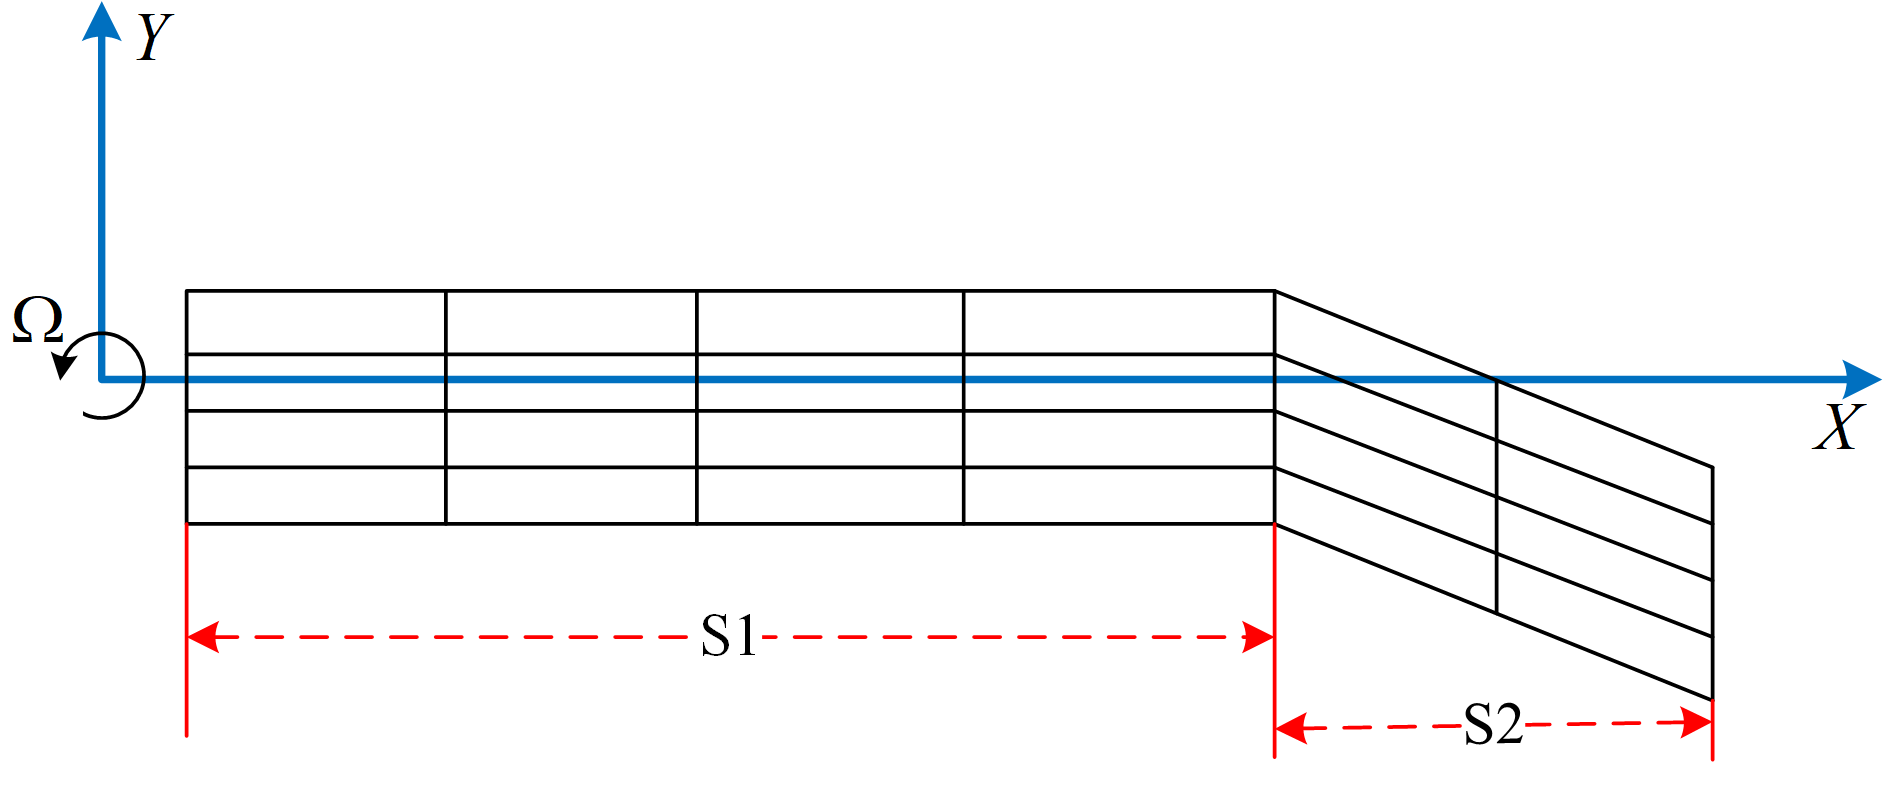
\includegraphics[width=7cm]{fig/figure_chap2/chap_2_5_2_1.png}
    \caption{带后掠的桨叶涡面网格划分}
    \label{fig:chap2_5_2_1}
  \end{figure}

将叶片沿展向分为几列,沿弦向分为几行,那么叶片表面将被划分为若干网格。虽然每个叶片段的展向编号不同,但弦向编号应保持不变。叶片的中弧面由涡四边形代替,涡四边形的展向附涡位于网格的四分之一弦线上,弦向附涡沿展向网格分布。在网格边界处,涡四边形的后缘涡位于相邻网格的四分之一弦线上。在叶片的后缘上,涡格等效地生成涡粒子团,如图\ref{fig:chap2_5_2_2}所示。

\begin{figure}[!htb]
    \centering
    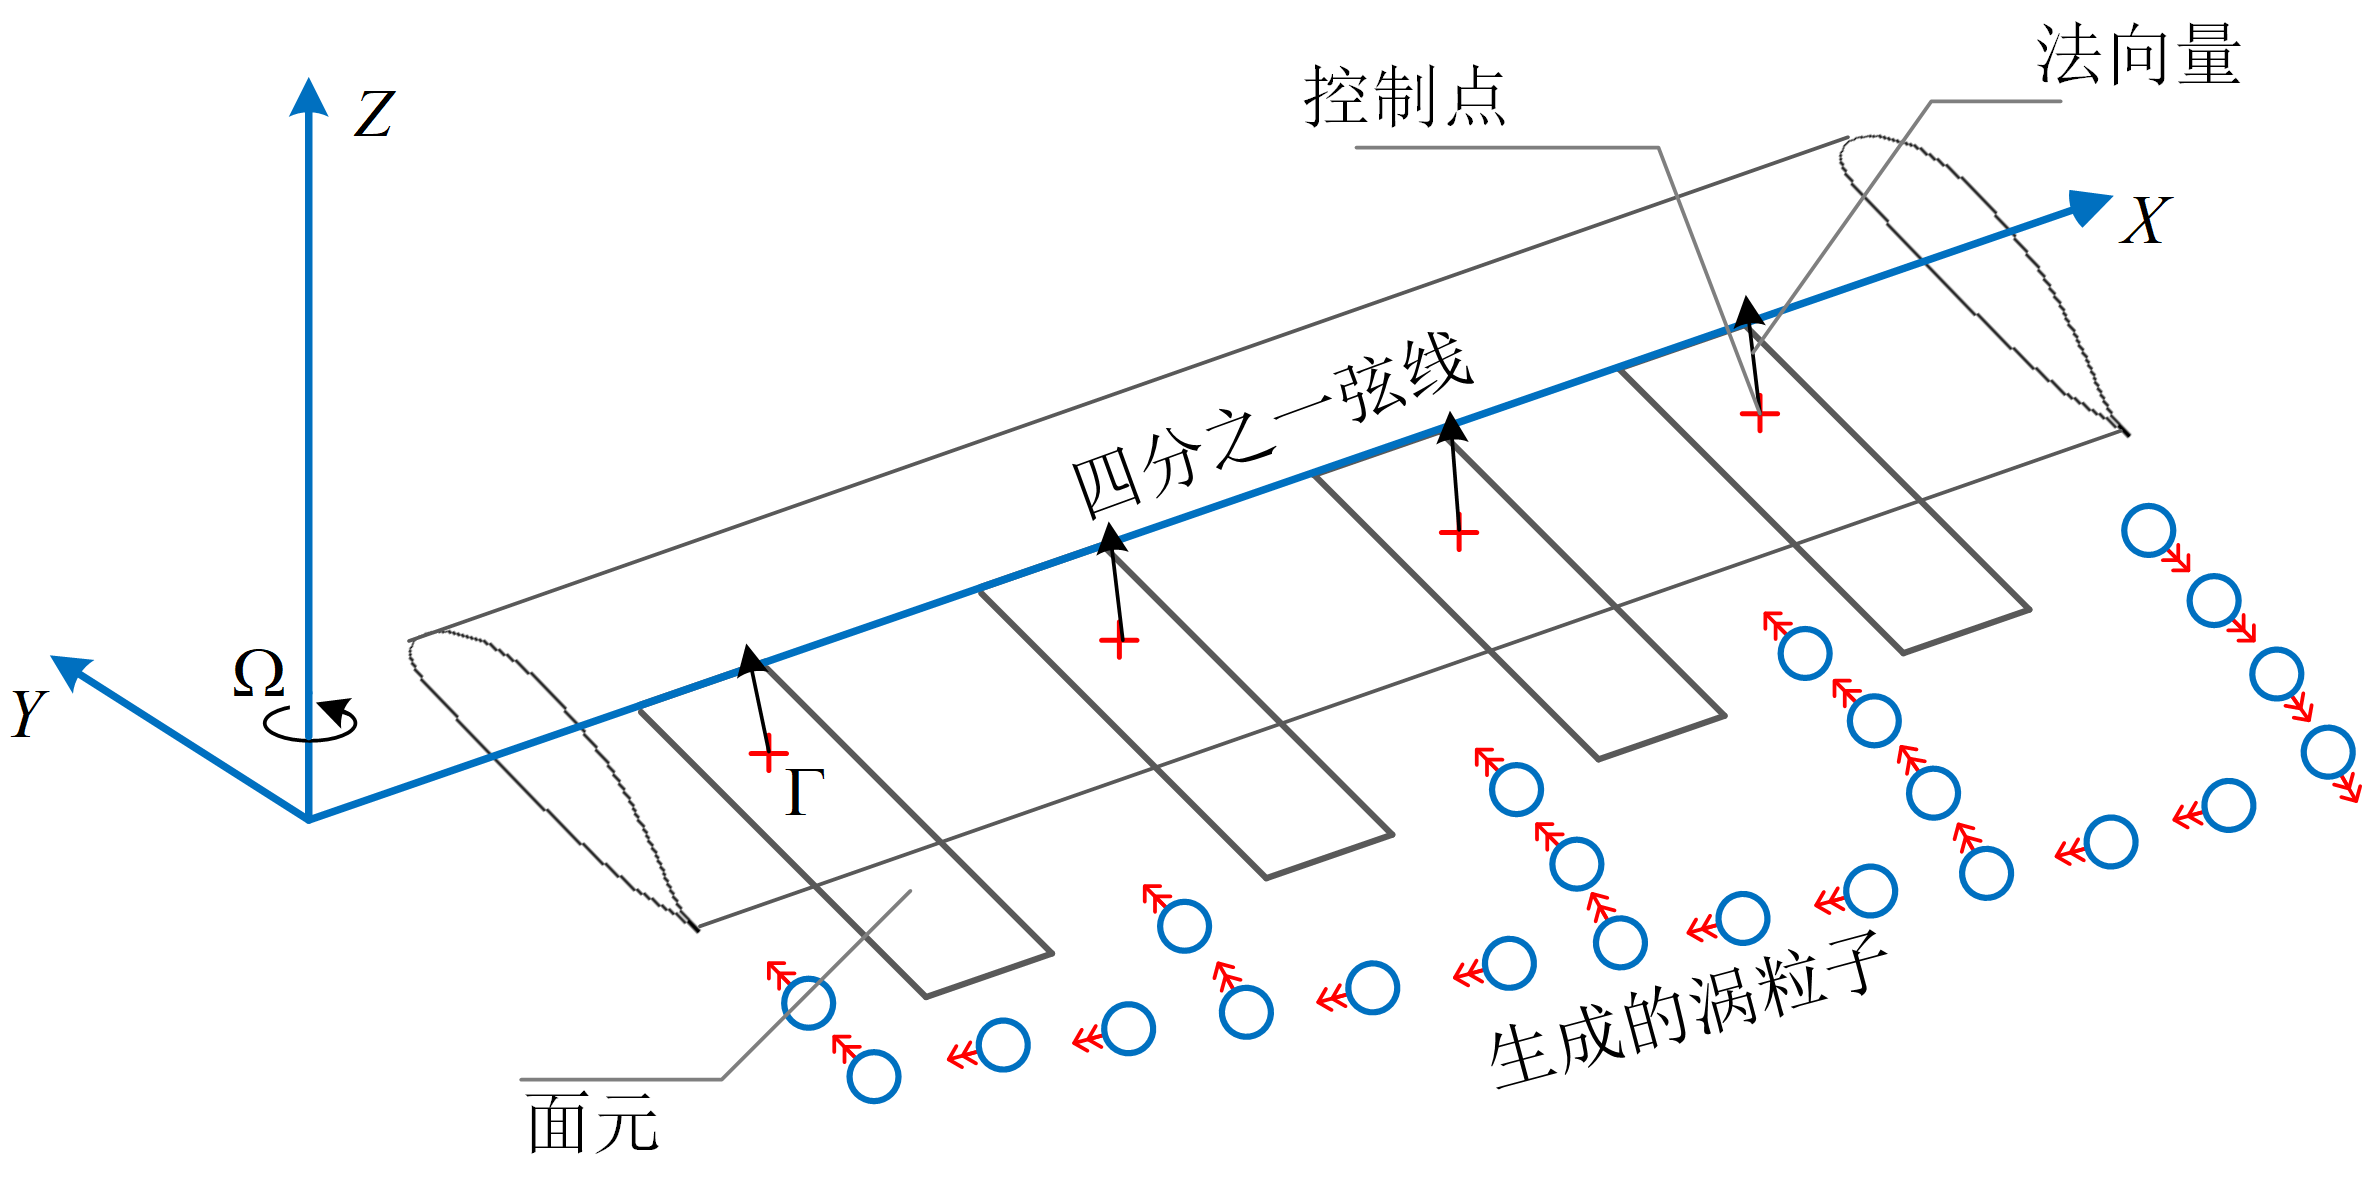
\includegraphics[width=7cm]{fig/figure_chap2/chap_2_5_2_2.png}
    \caption{桨叶上的涡元分布和后缘涡粒子生成示意图}
    \label{fig:chap2_5_2_2}
  \end{figure}

在每个叶片段后缘会产生涡源,并脱落到旋翼尾迹中。其中,涡源可以通过下式计算
\begin{equation}
    {r_{wake}} =  - \frac{{d{{\vec \Gamma }_b}}}{{dt}} + {\vec v_b}\nabla  \cdot {\vec \Gamma _b}
\end{equation}
其中,${r_{wake}}$为新产生的涡的强度。${\vec \Gamma _b}$是叶片约束环量的矢量形式。${\vec v_b}$是包含桨叶运动速度、远方来流速度、诱导速度、其他涡源干扰速度在内的当地合速度。在上面的公式中,第一项表示叶片约束环量的展向变化产生的尾涡,第二项表示叶片约束环量的方位变化产生的脱落涡。

\subsection{方法验证}
基于上述涡方法,对悬停状态下的Caradonna–Tung旋翼、前飞状态下的Scaled-model旋翼、以及纵列式双旋翼开展了分析。通过将计算结果与风洞试验数据进行对比,验证了本文建立的涡方法的有效性和可行性。

\begin{figure}[!htb]  
  \subfloat[$速度场$]{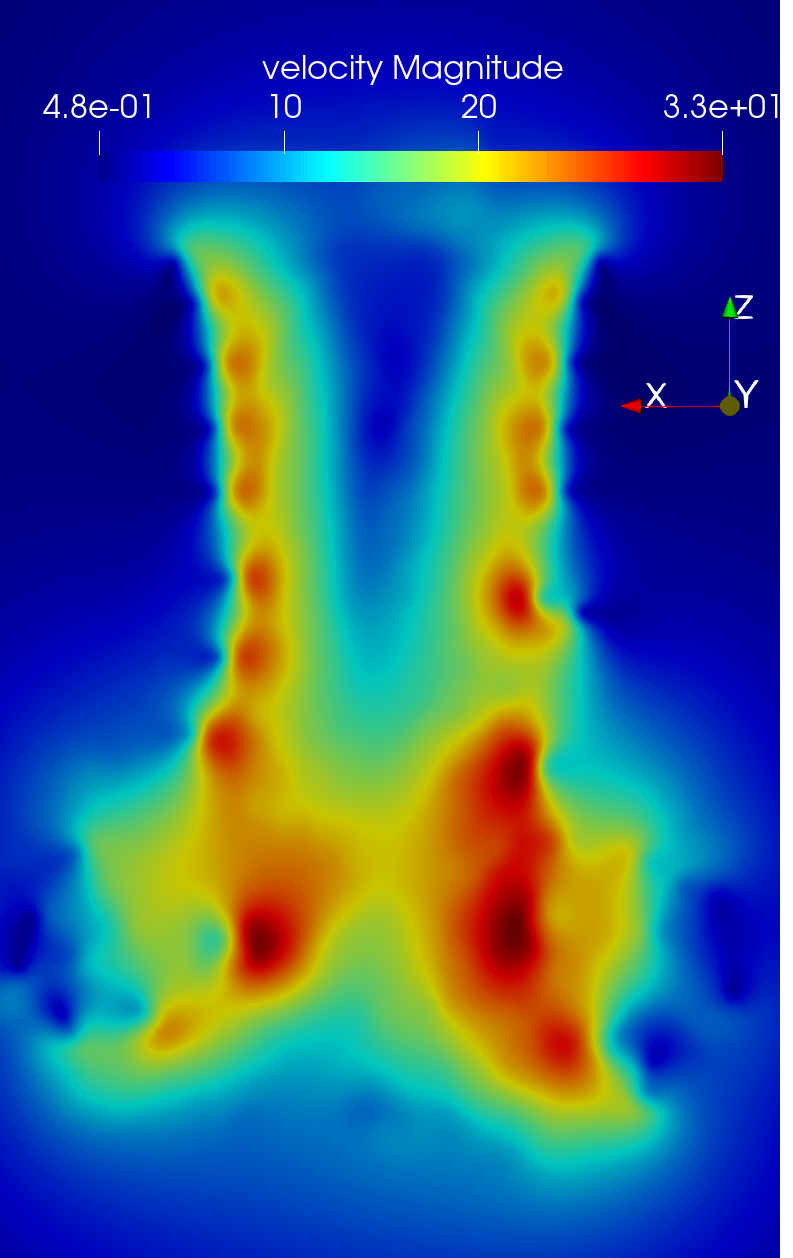
\includegraphics[width=4cm]{chap_2_5_3_1_1_1.png}}\quad
  \subfloat[$尾迹结构$]{\includegraphics[width=6cm]{chap_2_5_3_1_1_2.png}}\quad
  \subfloat[$涡度场$]{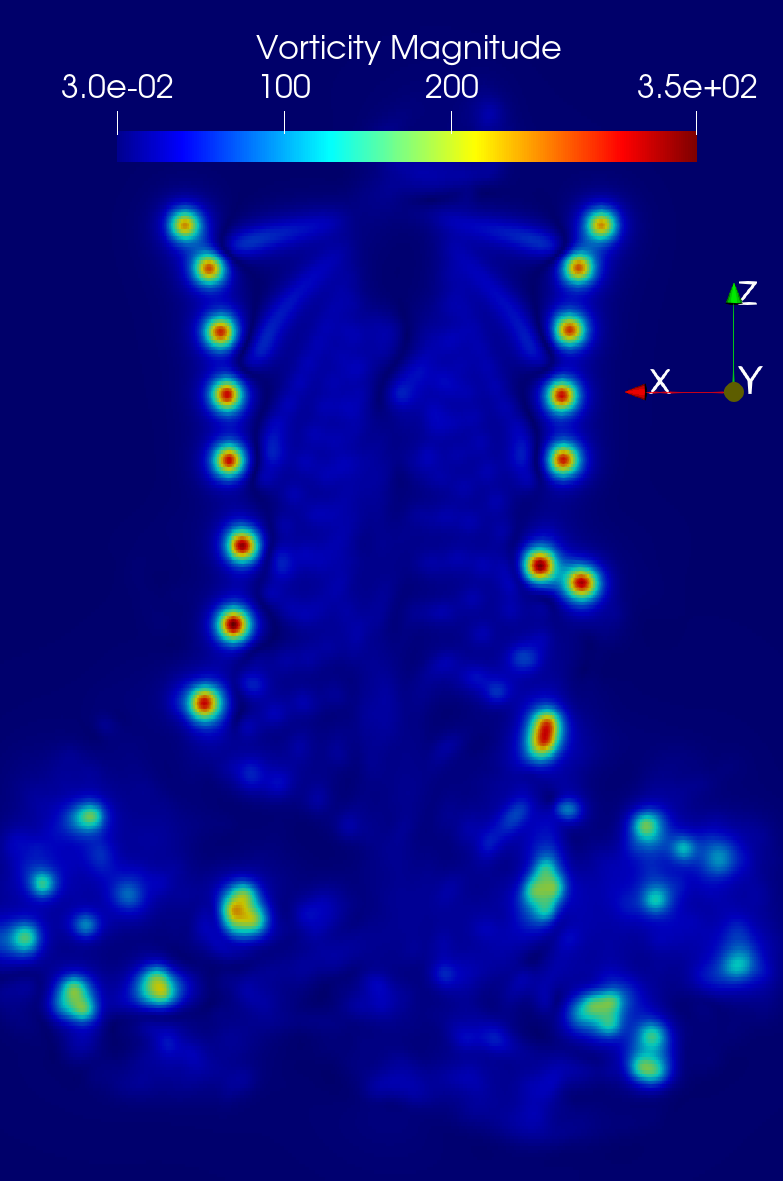
\includegraphics[width=4cm]{chap_2_5_3_1_1_3.png}}\quad\\
    \subfloat[$C_T$]{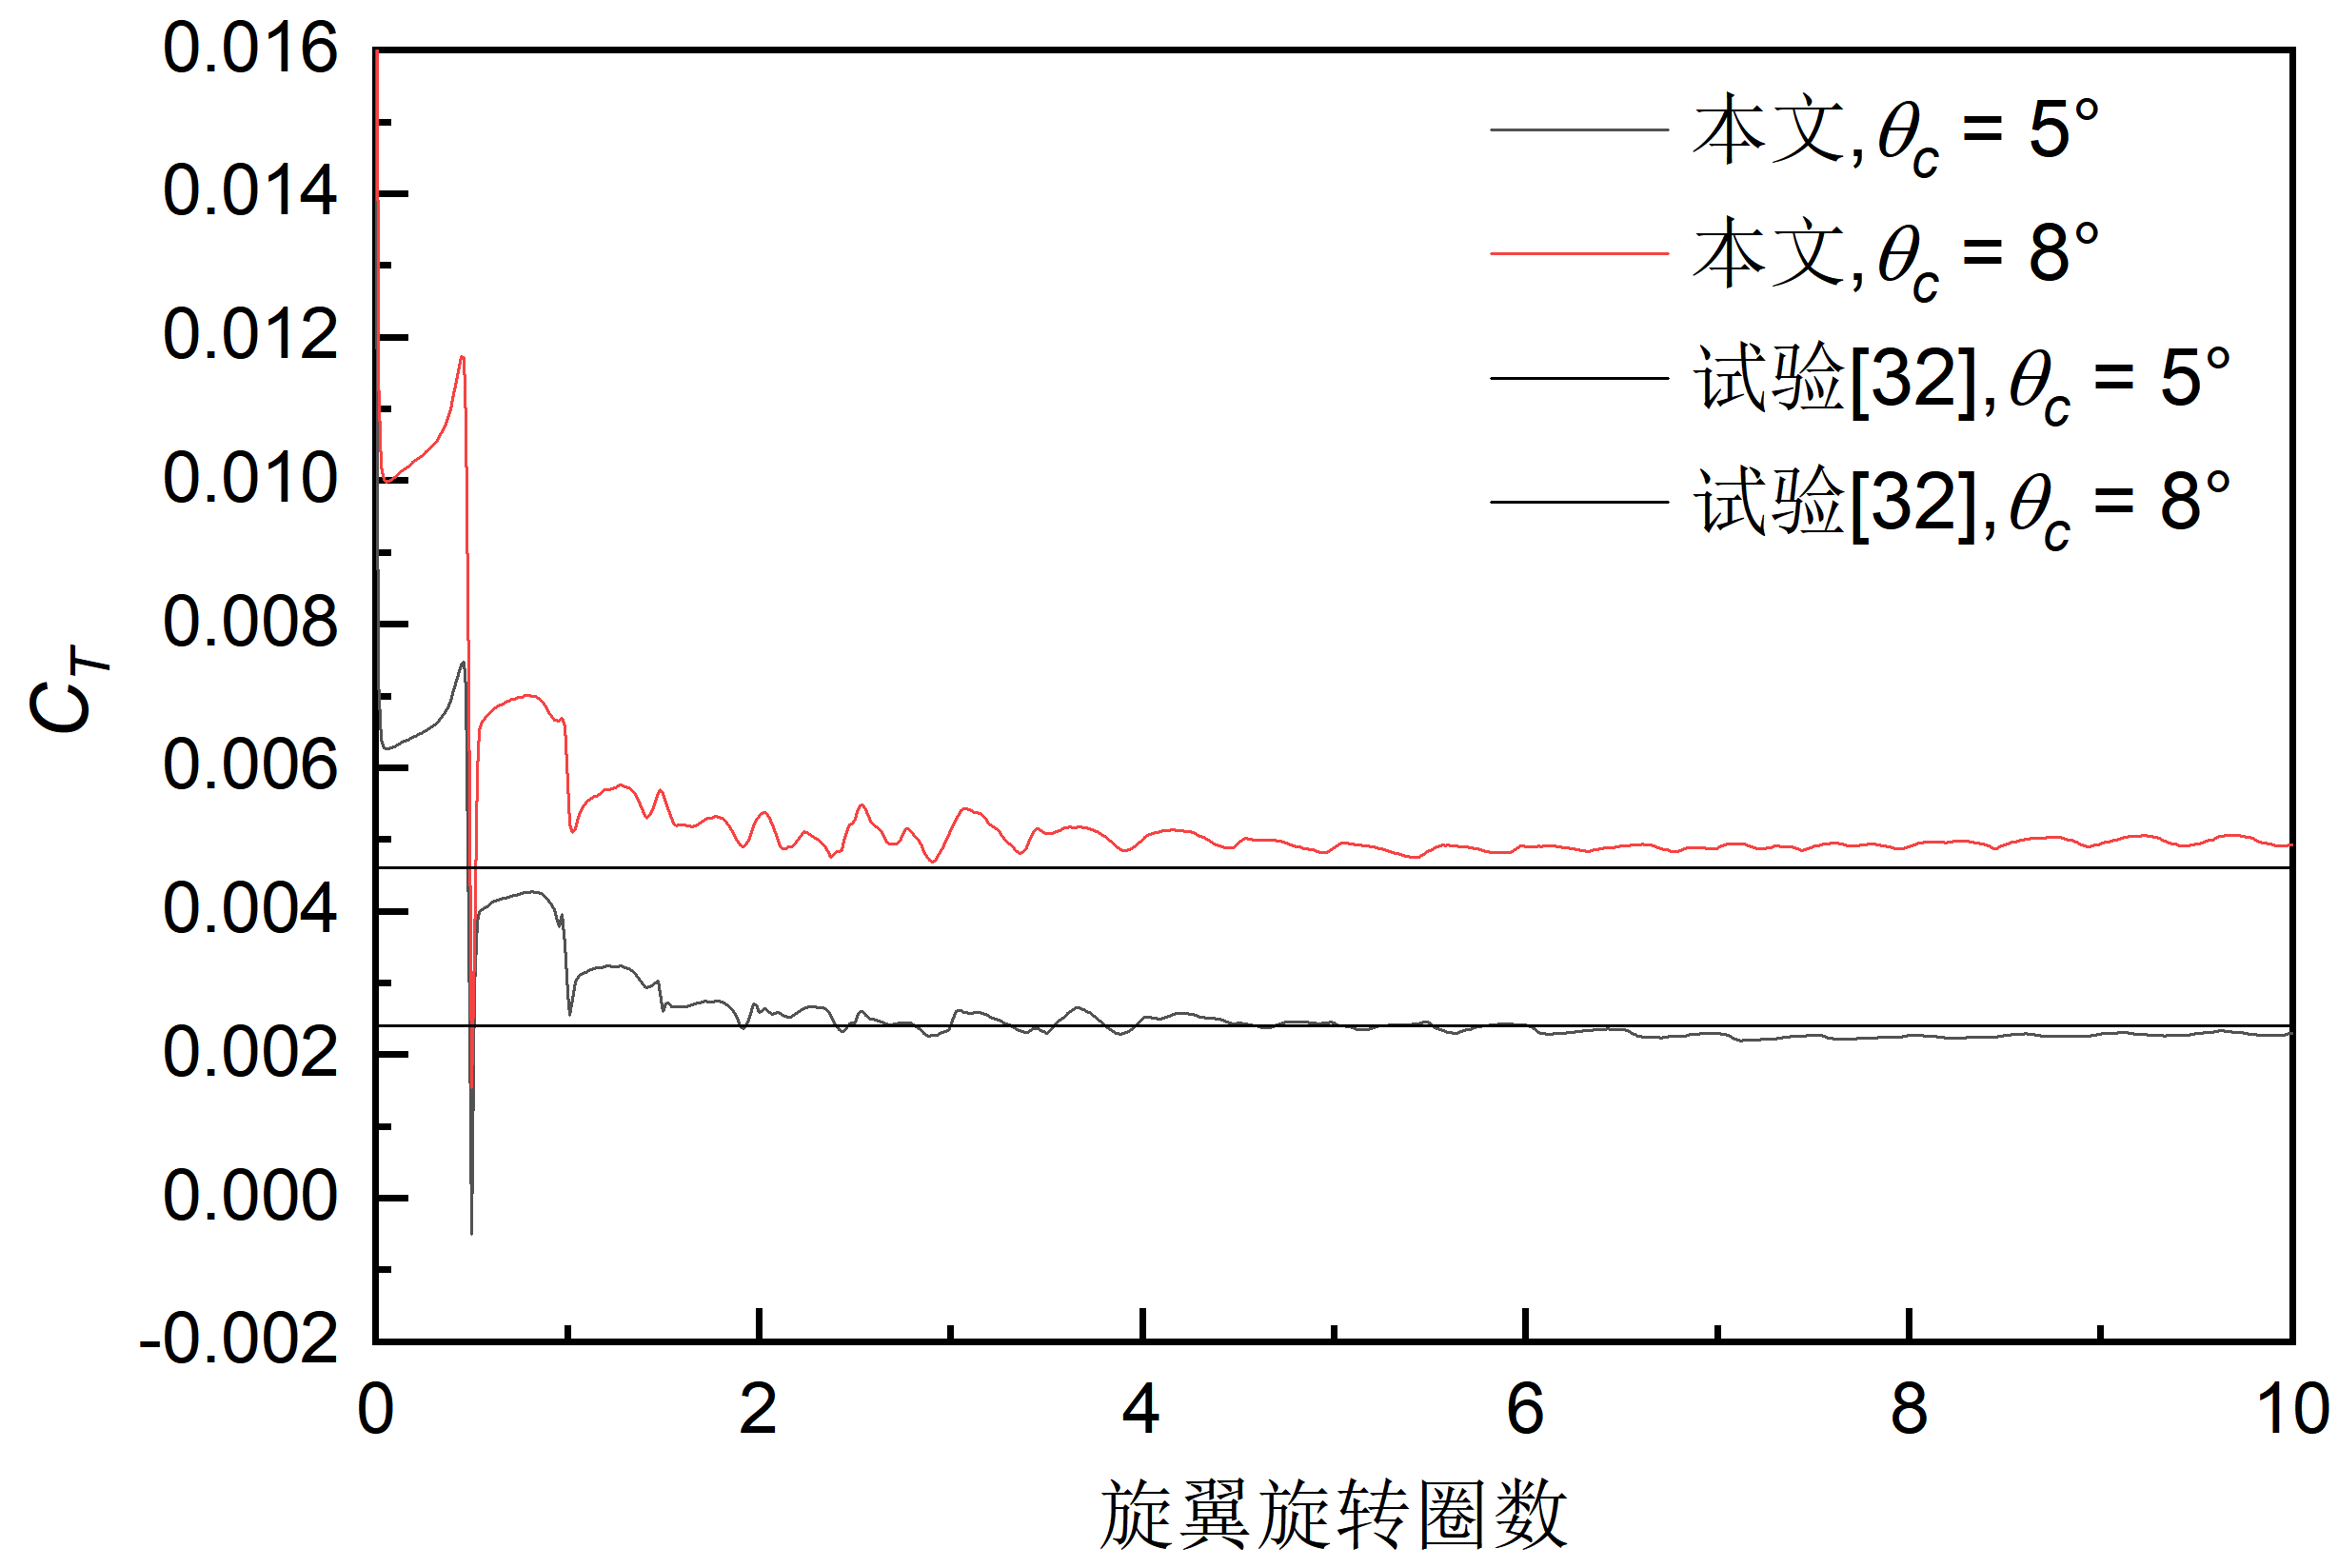
\includegraphics[width=7.3cm]{chap_2_5_3_1_2.png}}\quad
      \subfloat[升力系数]{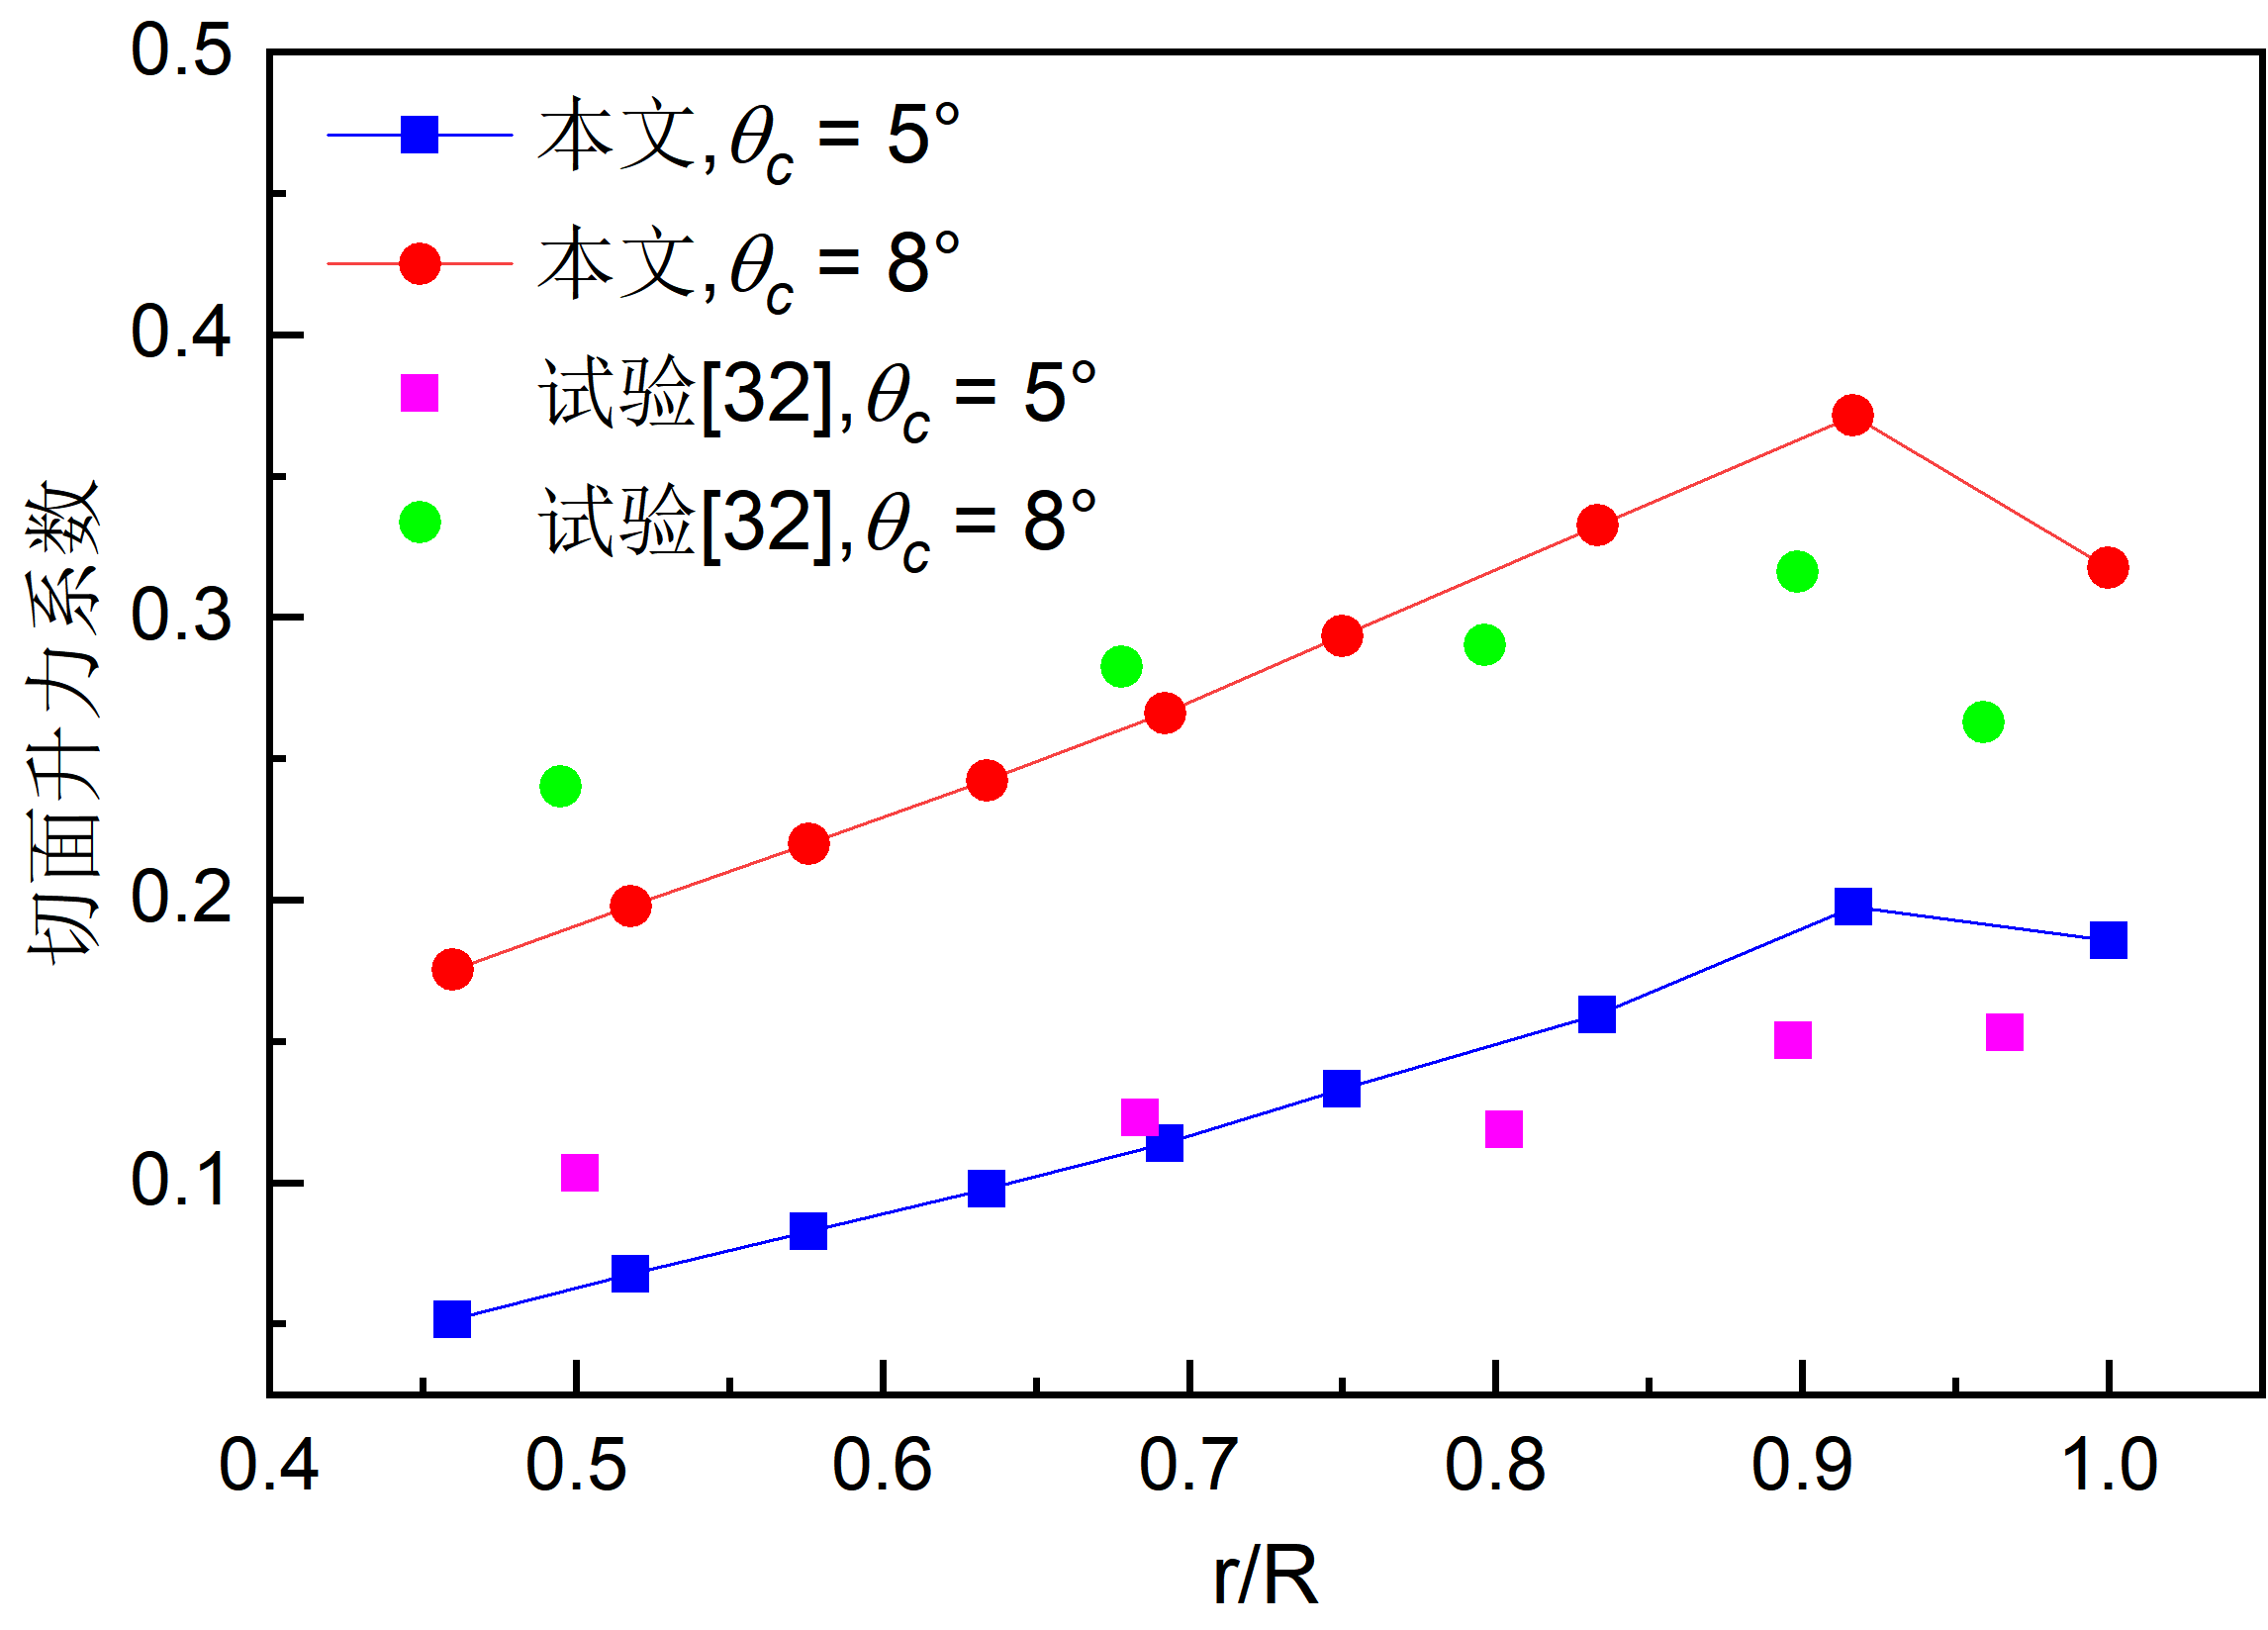
\includegraphics[width=7cm]{chap_2_5_3_1_3.png}}\\
      \caption{Caradonna–Tung旋翼计算结果与试验结果对比}
      \label{fig:chap2_5_3_1_2}
\end{figure}

\subsubsection{悬停状态下的Caradonna–Tung旋翼}
悬停状态下的Caradonna–Tung旋翼试验数据见参考文献\cite{caradonna1981experimental}。该旋翼有两片桨叶,桨叶翼型为NACA0012,无负扭、无尖削。旋翼半径为1.143 m,桨叶弦长为0.19 m,旋翼转速为1250 rpm。采取桨距为5 \degree 、8 \degree 时开展验证。

图\ref{fig:chap2_5_3_1_2}(a)-(c)给出了桨距为8 \degree 时旋翼旋转10圈后的速度场、尾迹结构、涡度场,可以清楚地捕捉到两片桨叶的桨尖涡和远场的管束区域,给出了尾迹的收缩、扩张、非周期、扩散、伸展运动。图\ref{fig:chap2_5_3_1_2}拉力系数的收敛过程。桨距为5 \degree 时,风洞试验拉力系数为0.0024;桨距为8 \degree 时,风洞试验拉力系数为0.0046。5个旋转周期后,计算值与试验值误差小于5 \%。图\ref{fig:chap2_5_3_1_2}给出了沿桨叶径向的载荷分布,基于涡方法计算得到的切面升力系数与试验值虽然有一定的差别,但整体趋势是一致的。

\begin{figure}[!htb]
  \centering
  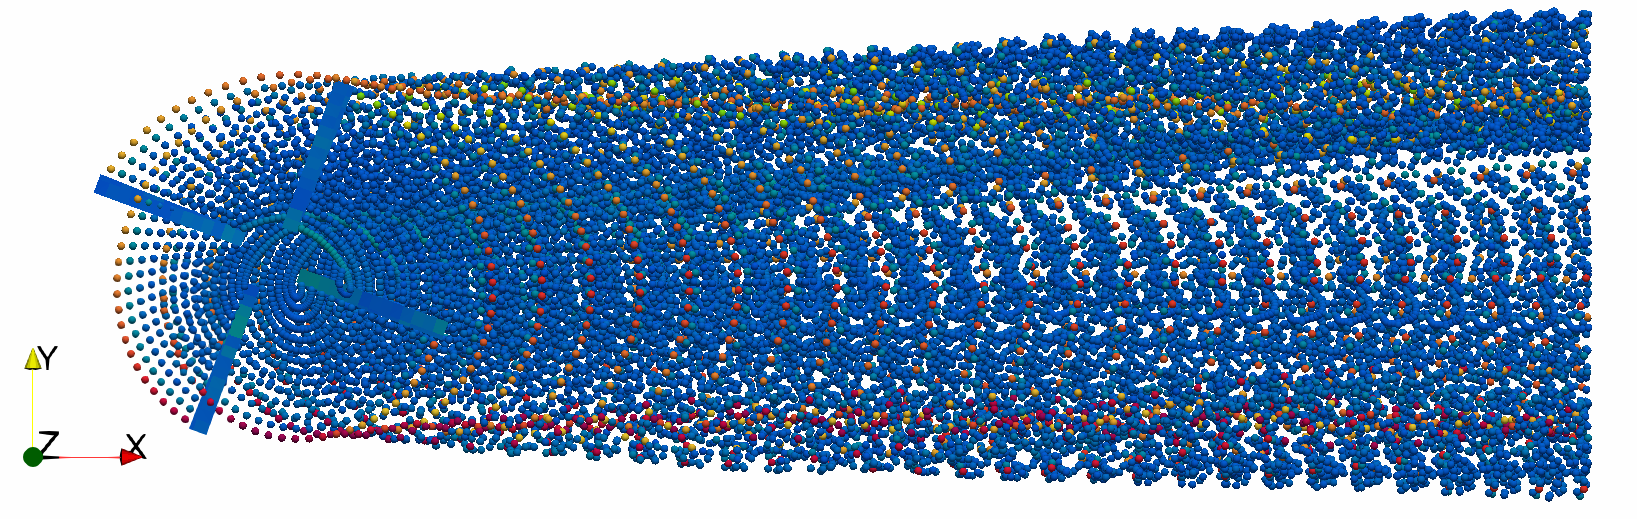
\includegraphics[width=10cm]{fig/figure_chap2/chap_2_5_3_2_1.png}
  \caption{前飞状态下的Scaled-model旋翼尾迹}
  \label{fig:chap2_5_3_2_1}
\end{figure}

\begin{figure}[!htb]  
  \subfloat[纵向入流速度]{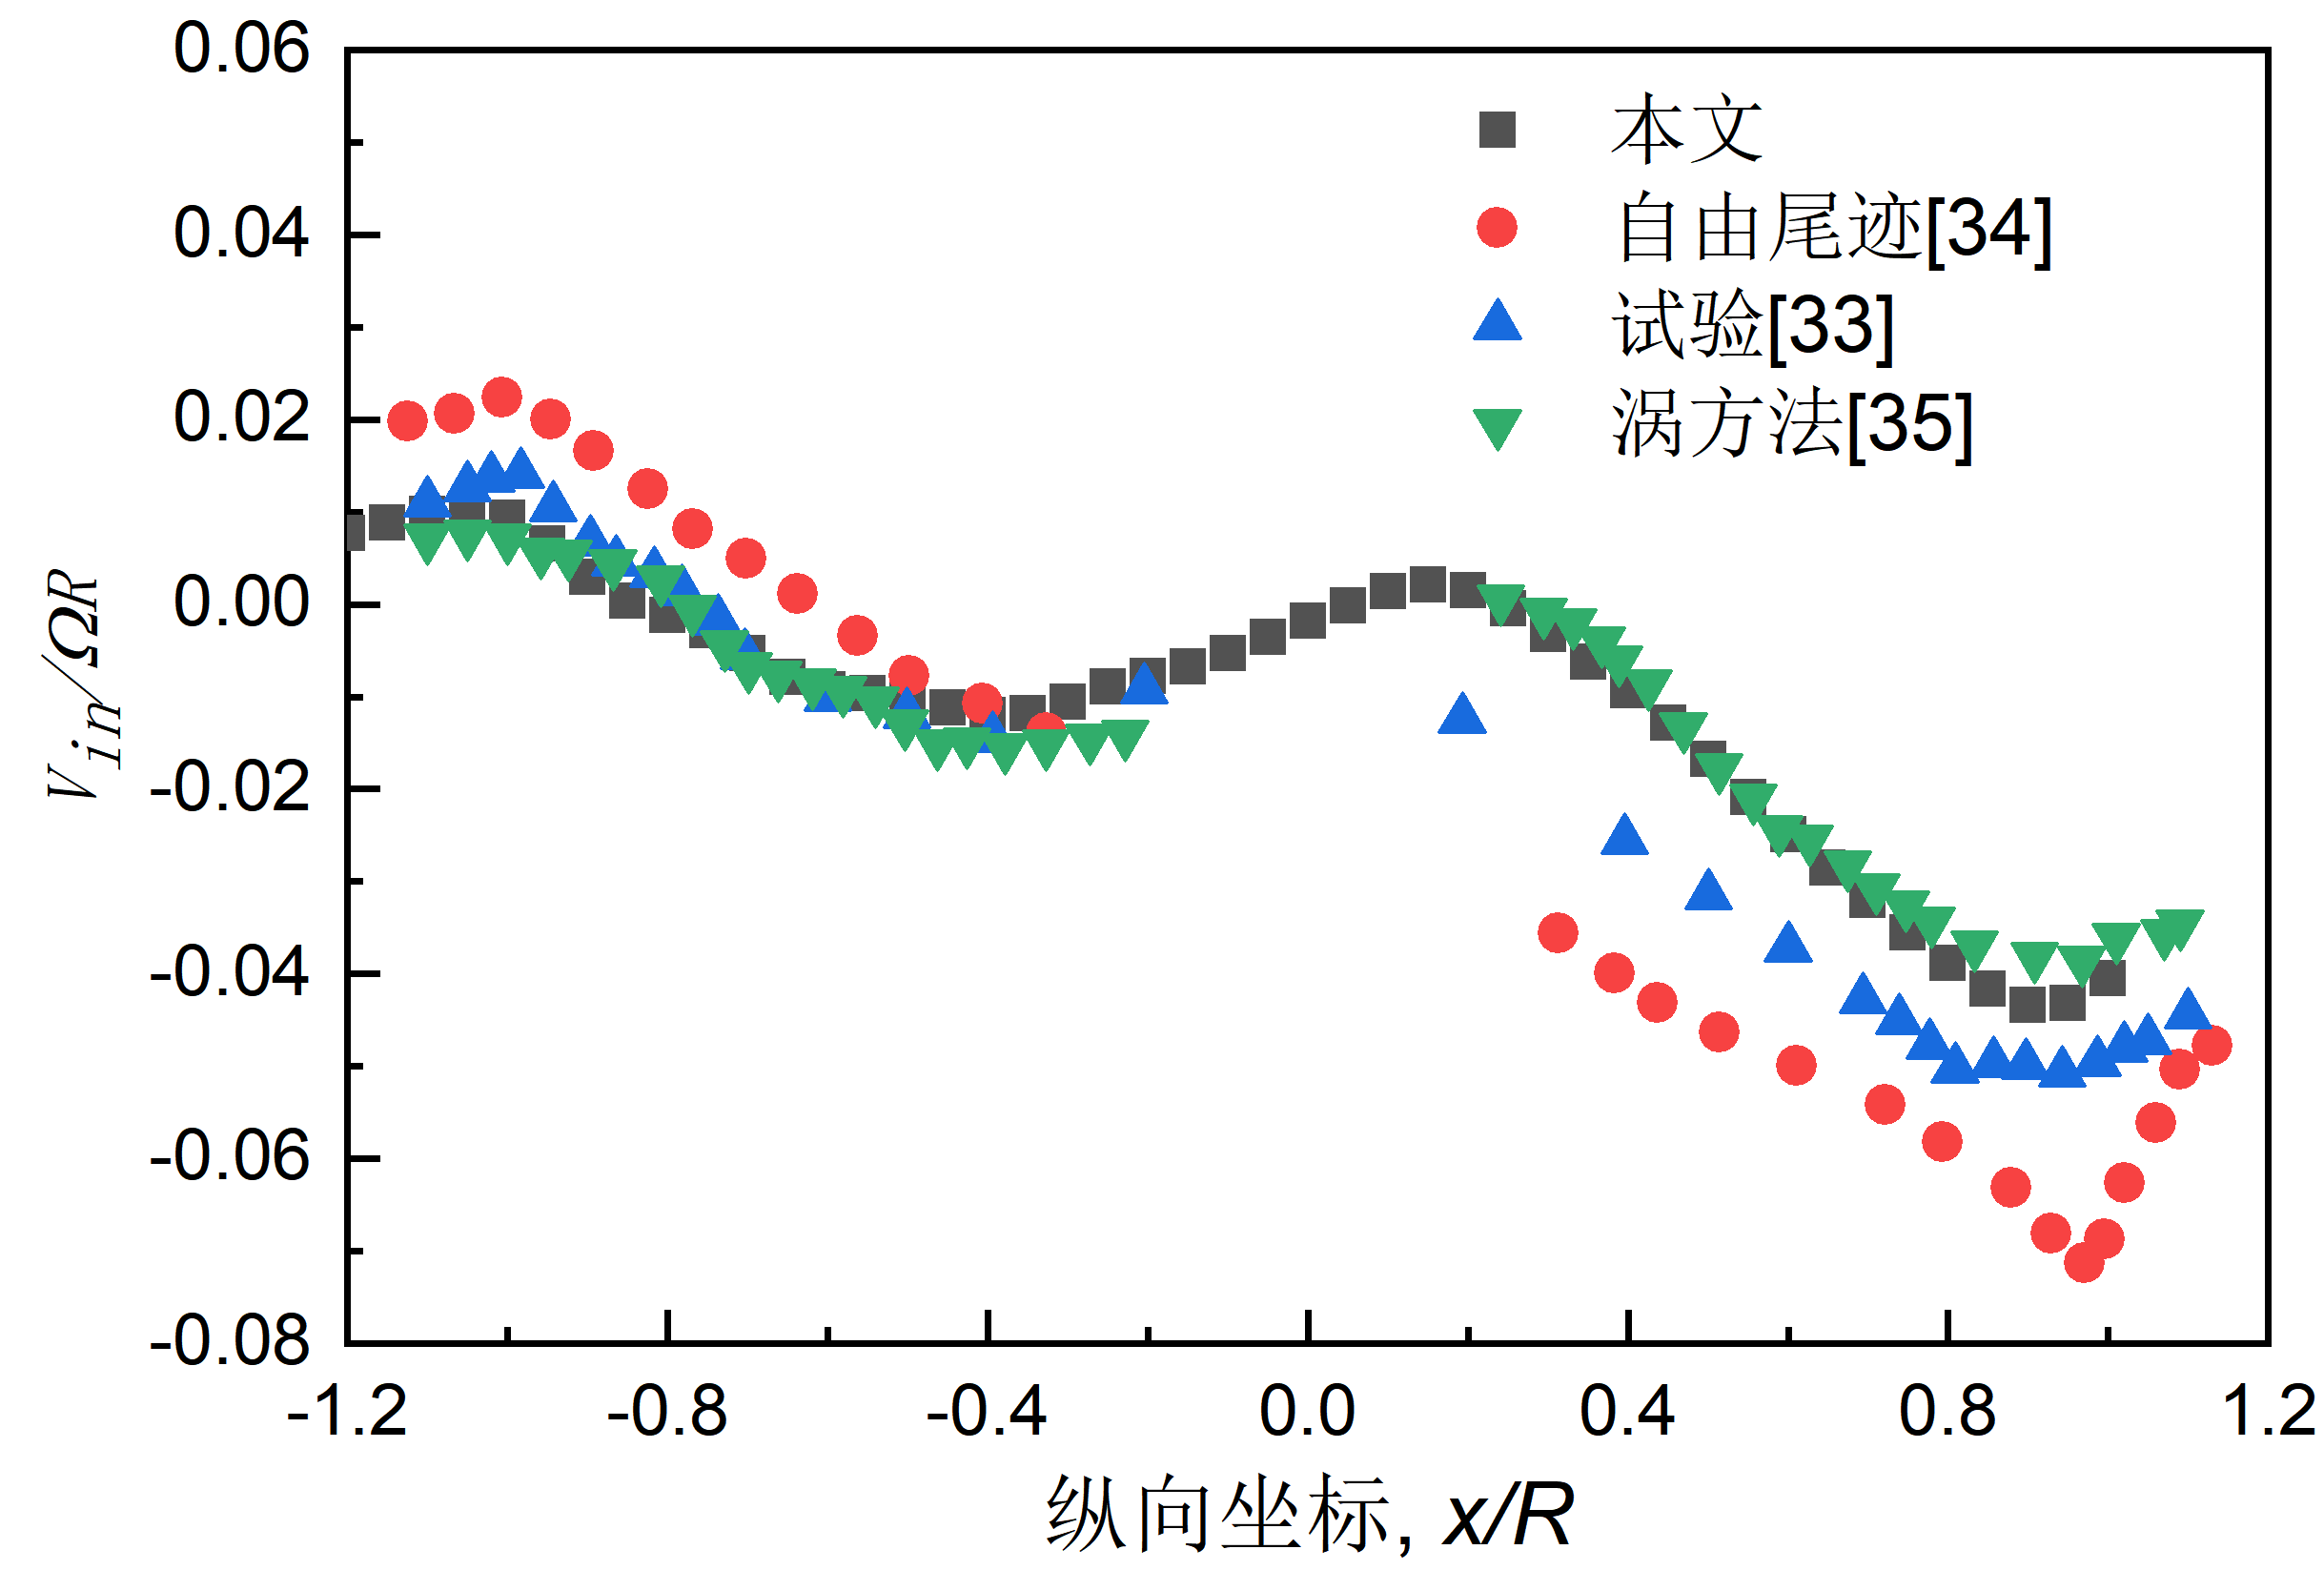
\includegraphics[width=7cm]{chap_2_5_3_2_2.png}}\quad
    \subfloat[横向入流速度]{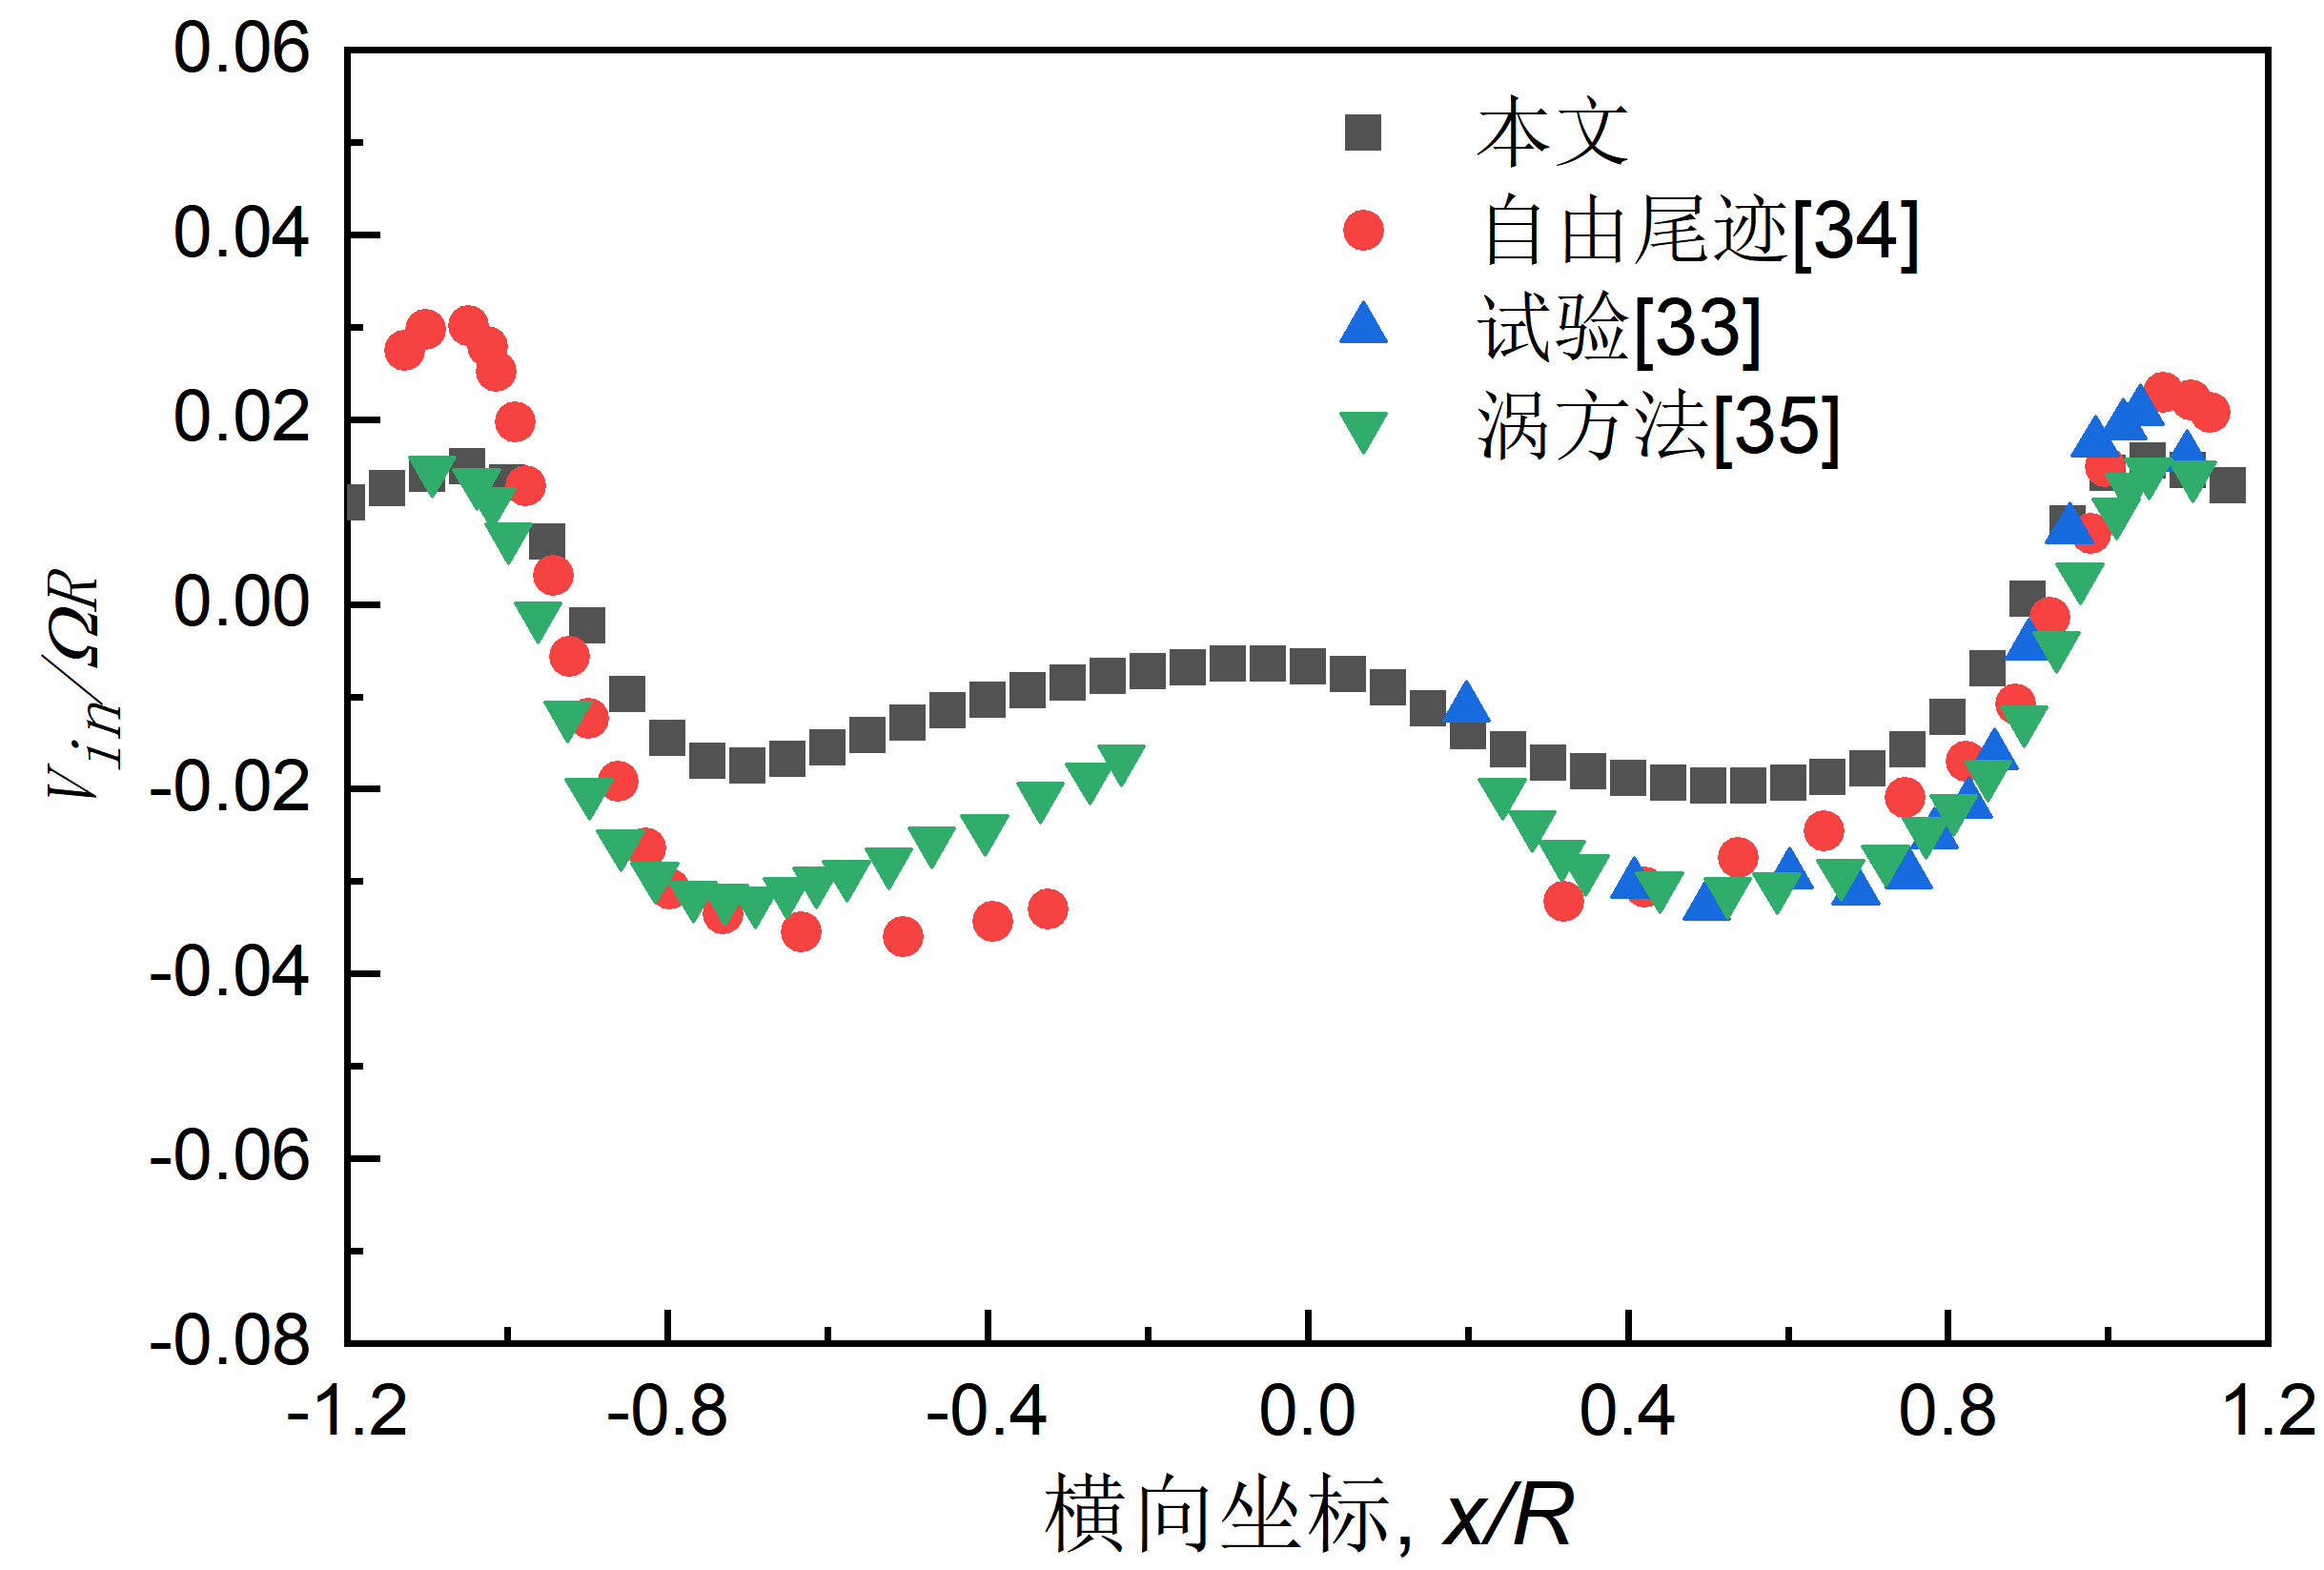
\includegraphics[width=7cm]{chap_2_5_3_2_3.png}}\\
    \caption{Scaled-model旋翼计算结果与试验结果对比}
    \label{fig:chap2_5_3_2_2}
\end{figure}

\subsubsection{前飞状态下的Scaled-model旋翼}
Scaled-model旋翼的风洞试验数据见参考文献\cite{elliott1988inflow}。Scaled-model旋翼有4片桨叶,桨叶翼型为NACA0012。旋翼转速为2113 rpm,旋翼半径为0.861 m,桨叶弦长为0.066 m,线性负扭为-8\degree。将桨距写为傅里叶形式,其常数项、一阶余弦项、一阶正弦项分别为6.3\degree,-2.1\degree,2\degree。桨盘迎角为3\degree。前飞速度为28.5 m/s,对应前进比0.15。

前飞状态下的Scaled-model旋翼尾迹见图\ref{fig:chap2_5_3_2_1}。基于上述涡方法,可以捕捉到前行侧、后行侧的初始桨尖涡以及后缘卷起的桨尖涡。

图\ref{fig:chap2_5_3_2_2}给出了纵向、横向的入流速度。与基于自由尾迹的计算结果\cite{bhagwat2001transient}相比,本文结果与试验值间误差更小。此外,可以看出,本文结果与参考文献\cite{tan2013simulating}中的结果基本一致,这也体现了本文提出的涡方法的有效性和可行性。

\subsubsection{纵列式双旋翼}
本文用来验证的纵列式双旋翼试验数据来自参考文献\cite{dingeldein1954wind}。其中,纵列式双旋翼两旋翼轴间的纵向距离为4.724 m,垂向、侧向距离均为0。前后旋翼桨叶无负扭、无尖削,翼型为NACA0012。旋翼半径为2.286 m,实度为0.054。
\begin{figure}[!htb]  
  \subfloat[悬停]{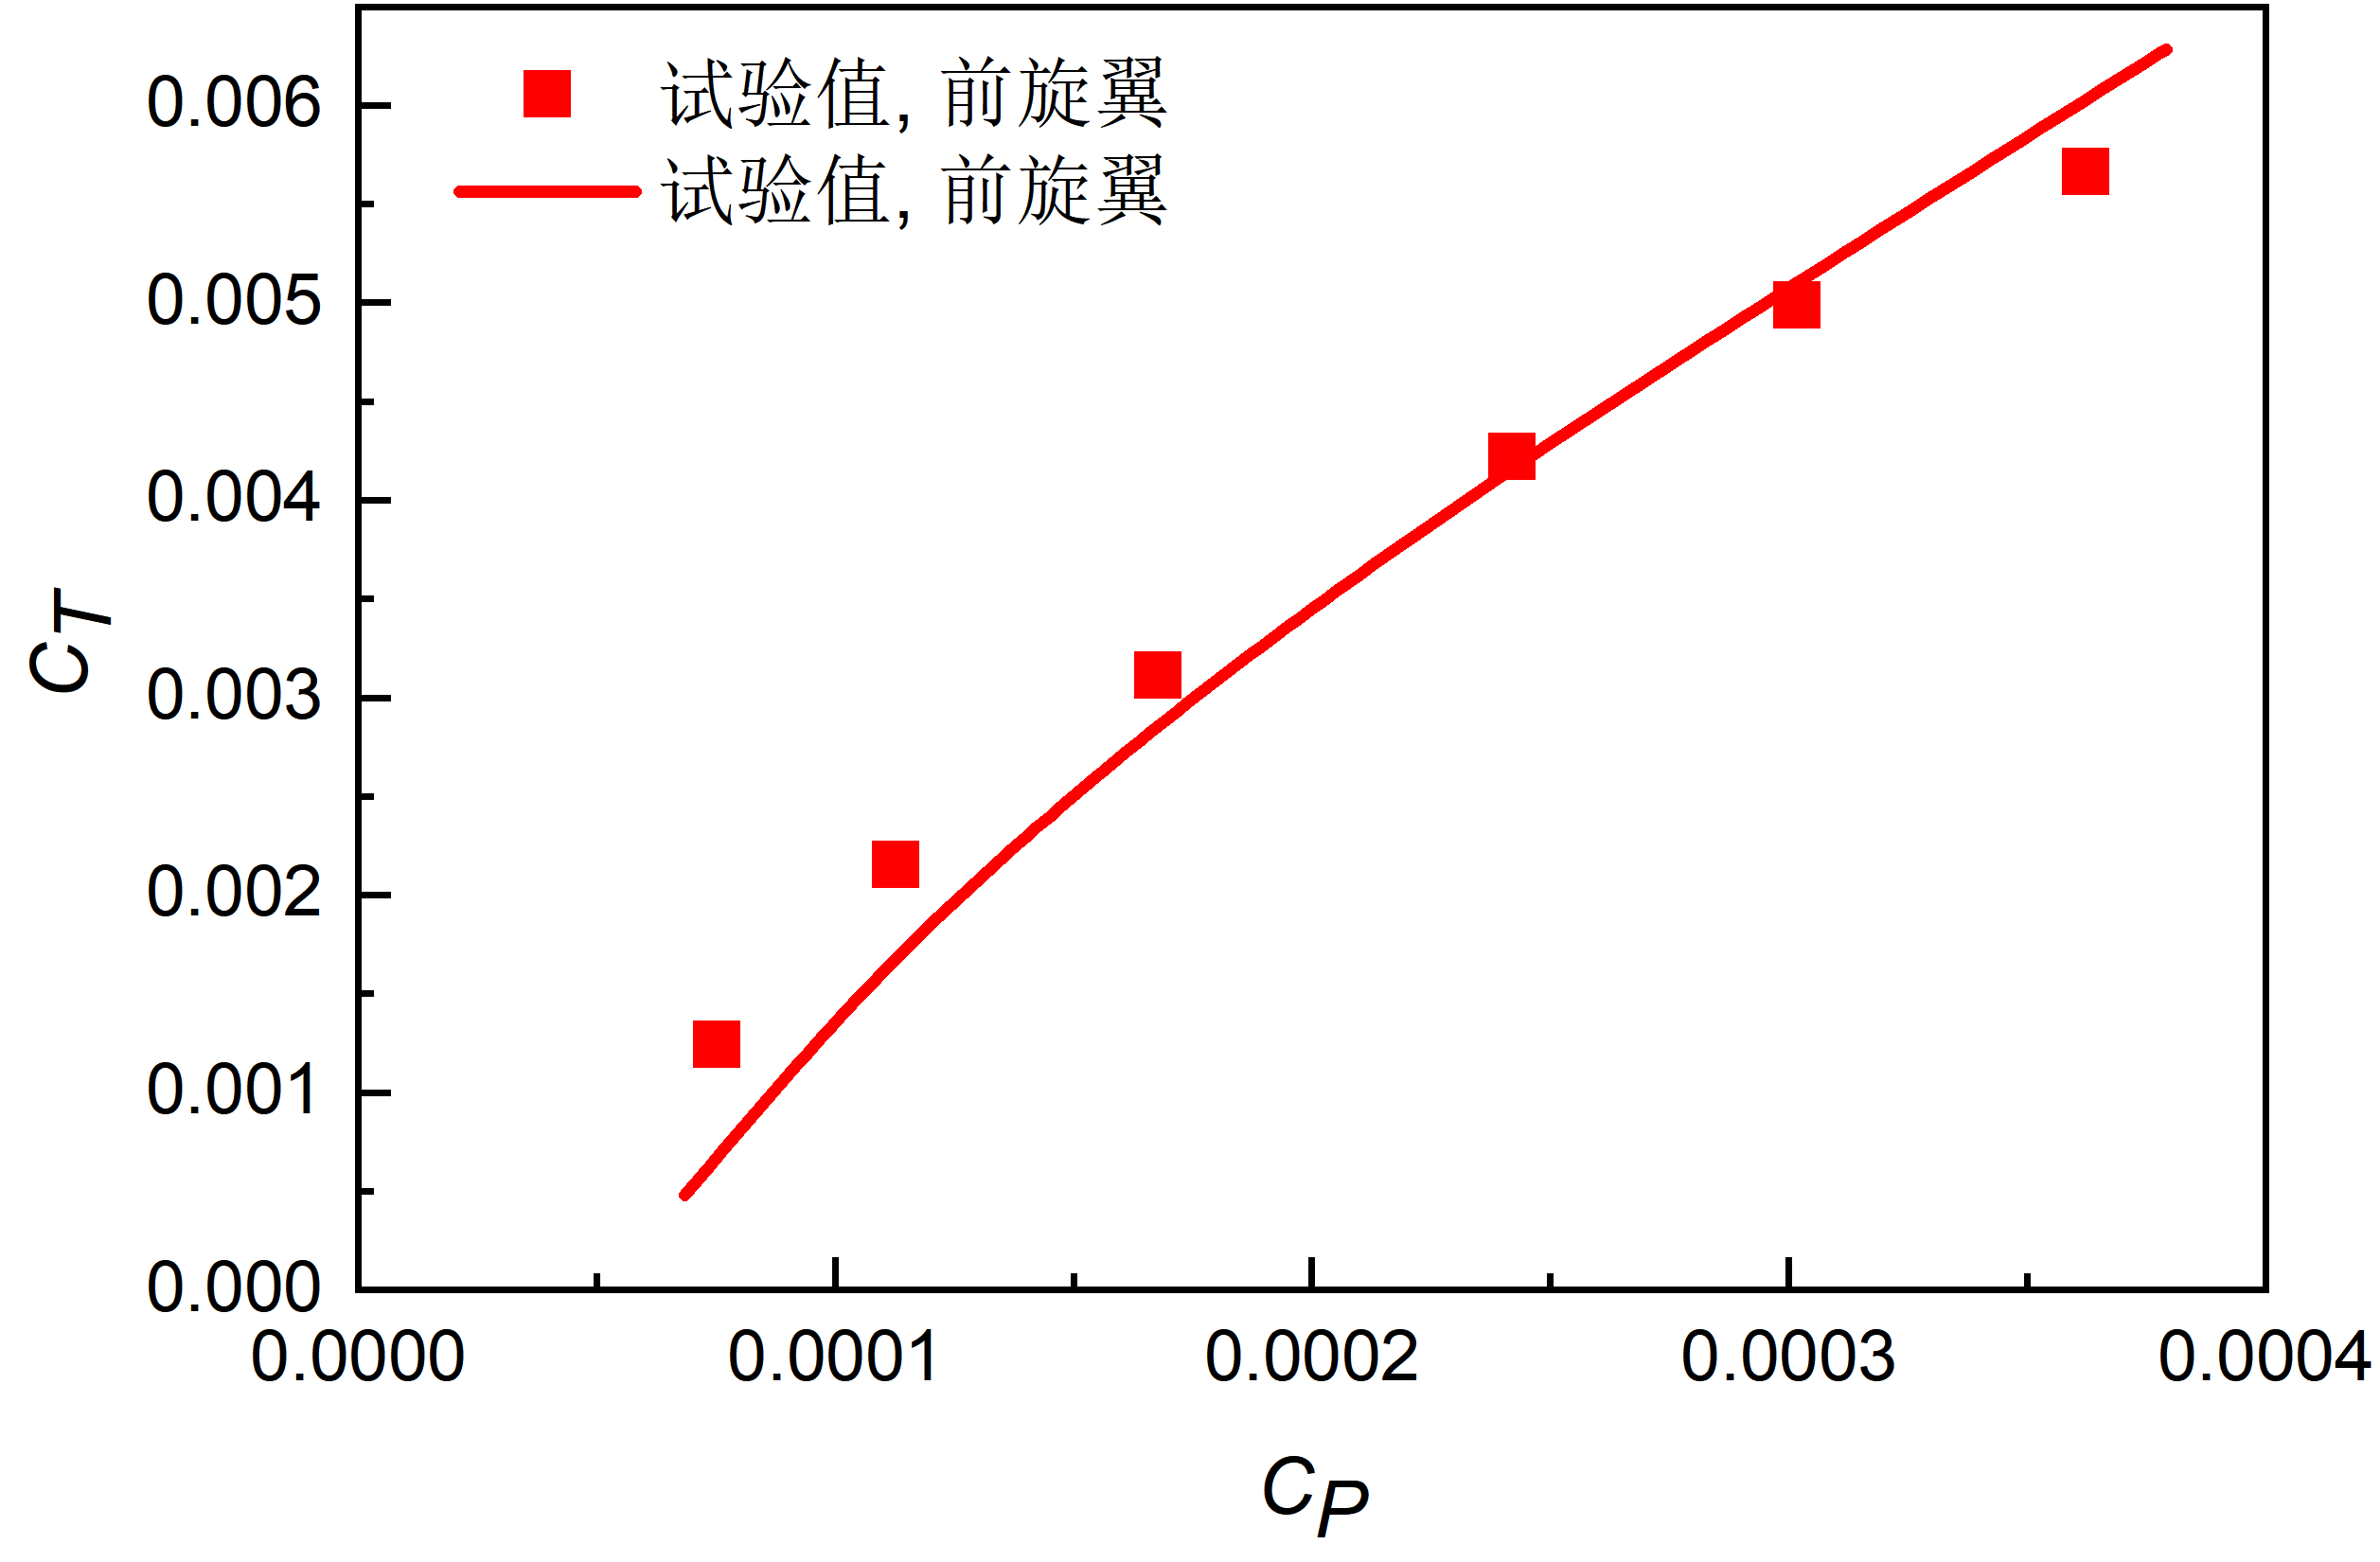
\includegraphics[width=7cm]{chap_2_5_3_3_1.png}}\quad
    \subfloat[定常平飞,$C_T=0.0034$]{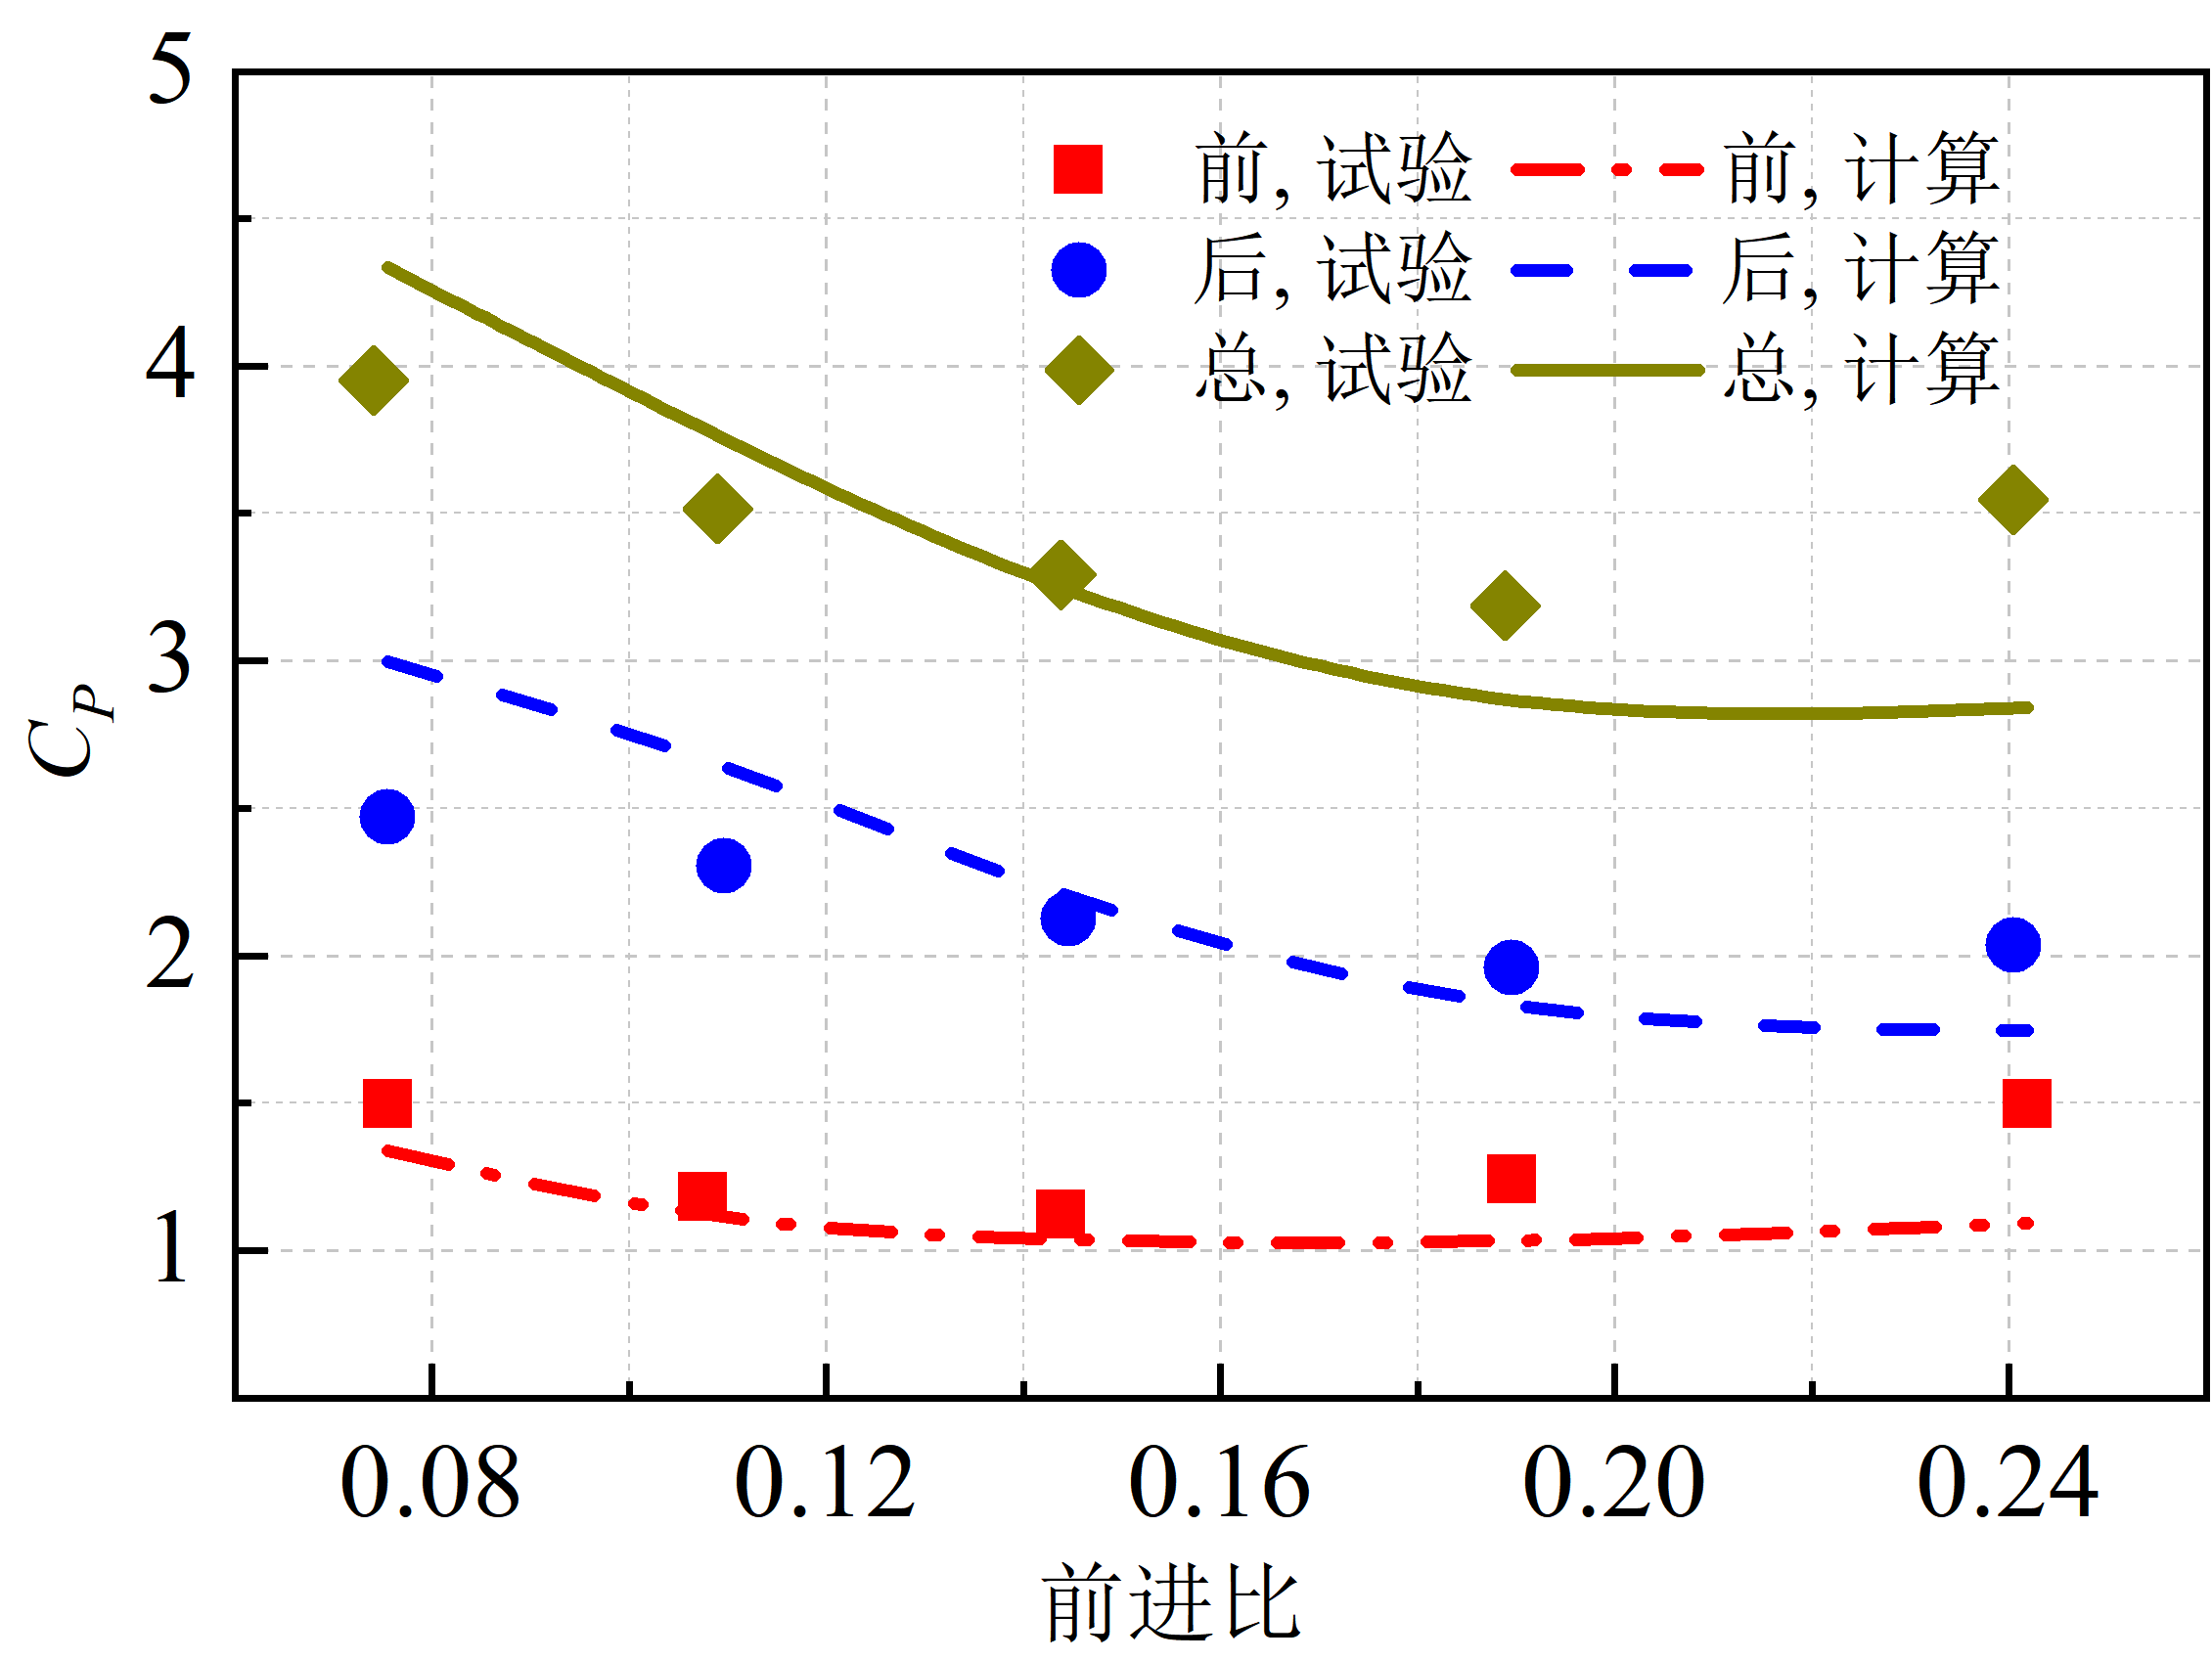
\includegraphics[width=6.7cm]{chap_2_5_3_3_2.png}}\\
    \caption{纵列式双旋翼计算结果与试验结果对比}
    \label{fig:chap2_5_3_3_1}
\end{figure}

考虑到悬停时前后旋翼位置对称、入流相等,前后旋翼性能一致。因此悬停时本文以前旋翼为例开展了分析,见图\ref{fig:chap2_5_3_3_1}(a)。可以看出,当$C_P$大于0.015时,基于涡方法计算得到的$C_T$与试验值间的相对误差小于10\%。$C_T$、$C_P$的值较小时,尽管相对误差较大,但计算值和试验值的整体趋势是一致的。

见图\ref{fig:chap2_5_3_3_1}(b),前飞时以$C_T$等于0.0034时的计算值与试验值为例开展对比分析。总功率消耗为前后旋翼功率消耗的和。可以看出,后旋翼的功率消耗比前旋翼的大,这是由于后旋翼除了受到自由流场作用外,还受到前旋翼的下洗流干扰。此外,当前进比大于0.2时,虽然前旋翼功率与试验结果之间相对误差较大,但整体趋势是一致的。

\section{直升机协同吊挂系统动力学模型}

\section{本章小结}